% Slide trình bày đồ án, Beamer, style UIT. Biên dịch: pdflatex bao-cao-do-an.tex (2 lần), hoặc tải thư mục slides/ lên Overleaf.
% Bật trang ghi chú thuyết trình: đổi \setbeameroption{hide notes} thành \setbeameroption{show notes}.
\documentclass[aspectratio=169,10pt]{beamer}
\usepackage[utf8]{vietnam}
\usepackage{lmodern}
\usepackage{array,booktabs,adjustbox,colortbl}
\usepackage[table]{xcolor}
\usetheme{UIT}
\ifdefined\shownotes\setbeameroption{show notes}\else\setbeameroption{hide notes}\fi
\title[Nhận diện giống chuối từ ảnh]{Nhận diện giống chuối từ ảnh}
\subtitle{Đồ án môn CS231.R12: Nhập môn Thị giác máy tính}
\author{Hoàng Quốc Duy \quad 24520373 \\ Nguyễn Thái Duy \quad 24520390 \\ Nguyễn Anh Khoa \quad 24520819}
\institute{}
\date{}
\begin{document}
\begin{frame}[plain]
\titlepage
\note{Kính chào thầy và các bạn. Nhóm em gồm ba thành viên: Hoàng Quốc Duy, Nguyễn Thái Duy, Nguyễn Anh Khoa. Hôm nay nhóm em xin trình bày đồ án nhận diện giống chuối từ ảnh. Bài trình bày đi theo thứ tự: lý do chọn đề tài, phát biểu bài toán, phương pháp, thực nghiệm, demo, rồi nhận xét và kết luận.}
\end{frame}
\section{Giới thiệu}
\begin{frame}{Lý do chọn đề tài}
\begin{columns}[T]
\begin{column}{0.56\textwidth}
\begin{itemize}\footnotesize
\item Chuối có nhiều giống, giá bán và cách dùng khác nhau; ở chợ, việc nhận ra giống vẫn làm bằng mắt
\item \textbf{BananaImageBD}: ảnh 4 giống chuối phổ biến ở Bangladesh, thu tại chợ đầu mối và cửa hàng, hướng tới ứng dụng nông nghiệp và chuỗi cung ứng
\item Phù hợp để áp dụng kiến thức môn học:
\begin{itemize}
\item 4 giống khác nhau cả màu lẫn hình dạng: so sánh được đặc trưng màu với hình dạng
\item Dữ liệu nhỏ (2471 ảnh), lệch lớp (2.2 lần): thấy rõ quá khớp, lợi ích của transfer learning
\item Ảnh một quả trên nền trơn: kiểm tra được mô hình nhìn quả hay nhìn nền
\end{itemize}
\item \textbf{Cơ sở thực hiện:} dữ liệu công khai (CC BY 4.0); có bài báo đạt 99.70\% trên cùng dữ liệu để đối chiếu
\end{itemize}
\end{column}
\begin{column}{0.42\textwidth}
\begin{center}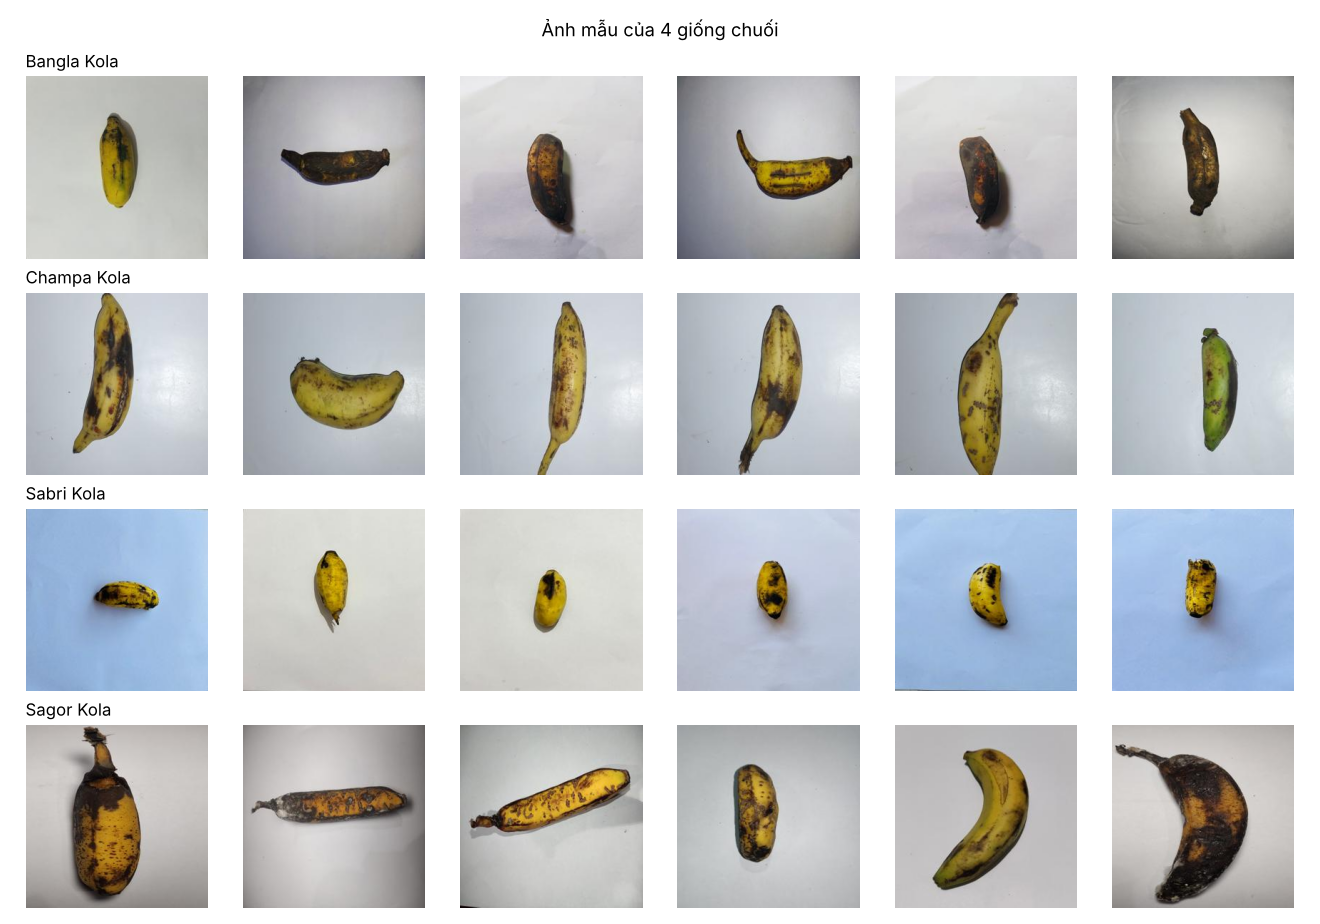
\includegraphics[width=\linewidth,height=0.72\textheight,keepaspectratio]{../results/figures/data_samples.png}\end{center}
\end{column}
\end{columns}
\note{Lý do thứ nhất là ý nghĩa thực tế. Chuối có nhiều giống, giá bán và cách dùng khác nhau, mà ở chợ người ta vẫn phân biệt bằng mắt và kinh nghiệm. Bộ dữ liệu BananaImageBD được thu ngay tại chợ đầu mối và cửa hàng ở Bangladesh, tác giả hướng tới ứng dụng trong nông nghiệp và chuỗi cung ứng. Lý do thứ hai là bài toán này hợp với môn học. Bốn giống khác nhau cả về màu lẫn hình dạng, nên nhóm em so sánh được đặc trưng màu với đặc trưng hình dạng. Dữ liệu nhỏ và lệch lớp, nên thấy rõ hiện tượng quá khớp và lợi ích của transfer learning. Ảnh chụp một quả trên nền trơn, nên kiểm tra được mô hình đang nhìn quả chuối hay nhìn nền. Về cơ sở thực hiện: dữ liệu công khai, có giấy phép, và đã có một bài báo công bố kết quả 99.70\% trên chính bộ dữ liệu này để nhóm em đối chiếu.}
\end{frame}

\begin{frame}{Phát biểu bài toán}
\textbf{Cho:}
\begin{itemize}
\item Tập nhãn $C=\{\text{Bangla Kola},\ \text{Champa Kola},\ \text{Sabri Kola},\ \text{Sagor Kola}\}$, số lớp $K=4$
\item Tập huấn luyện $D=\{(x_i,y_i)\}_{i=1}^{N}$: $x_i\in\{0,\dots,255\}^{256\times256\times3}$ là ảnh màu chụp một quả chuối, $y_i\in C$ là giống của quả chuối
\end{itemize}
\textbf{Tìm:} hàm phân loại $f$ sao cho với ảnh $x$ chưa gặp,
\[ f(x)=p=(p_1,p_2,p_3,p_4),\quad p_k\ge 0,\quad \sum_{k=1}^{4}p_k=1,\qquad \hat{y}=\arg\max_k p_k \ \text{trùng với nhãn thật } y \]
\begin{columns}[T]
\begin{column}{0.47\textwidth}
\begin{block}{Input}
Một ảnh màu $x$ chụp \textbf{một quả chuối} (chương trình tự đưa về $256\times256$)
\end{block}
\end{column}
\begin{column}{0.47\textwidth}
\begin{block}{Output}
Nhãn $\hat{y}\in C$ (tên giống) và vector xác suất $p$ của 4 lớp
\end{block}
\end{column}
\end{columns}
\vspace{1mm}
{\footnotesize \textbf{Ràng buộc:} đầu ra chỉ gồm 4 lớp, không có lớp ``khác''. Ảnh ngoài phạm vi (giống khác, không phải chuối) vẫn được gán vào một trong 4 giống.}
\note{Đây là bài toán phân loại ảnh nhiều lớp. Cho trước tập nhãn C gồm bốn giống chuối, và tập huấn luyện D gồm các cặp ảnh và nhãn, trong đó mỗi ảnh là ảnh màu 256 nhân 256 chụp một quả chuối. Cần tìm hàm phân loại f. Với một ảnh x chưa gặp, f trả về vector xác suất p gồm bốn thành phần không âm, tổng bằng một. Nhãn dự đoán là lớp có xác suất lớn nhất, và ta muốn nhãn này trùng với nhãn thật. Khi sử dụng, input là một ảnh màu chụp một quả chuối, output là tên giống và xác suất của bốn lớp. Nhóm em lưu ý một ràng buộc: đầu ra chỉ gồm bốn lớp, không có lớp khác. Nên nếu đưa vào ảnh ngoài phạm vi, chương trình vẫn chạy và vẫn trả về một trong bốn giống.}
\end{frame}

\begin{frame}{Hình minh họa bài toán}
\begin{center}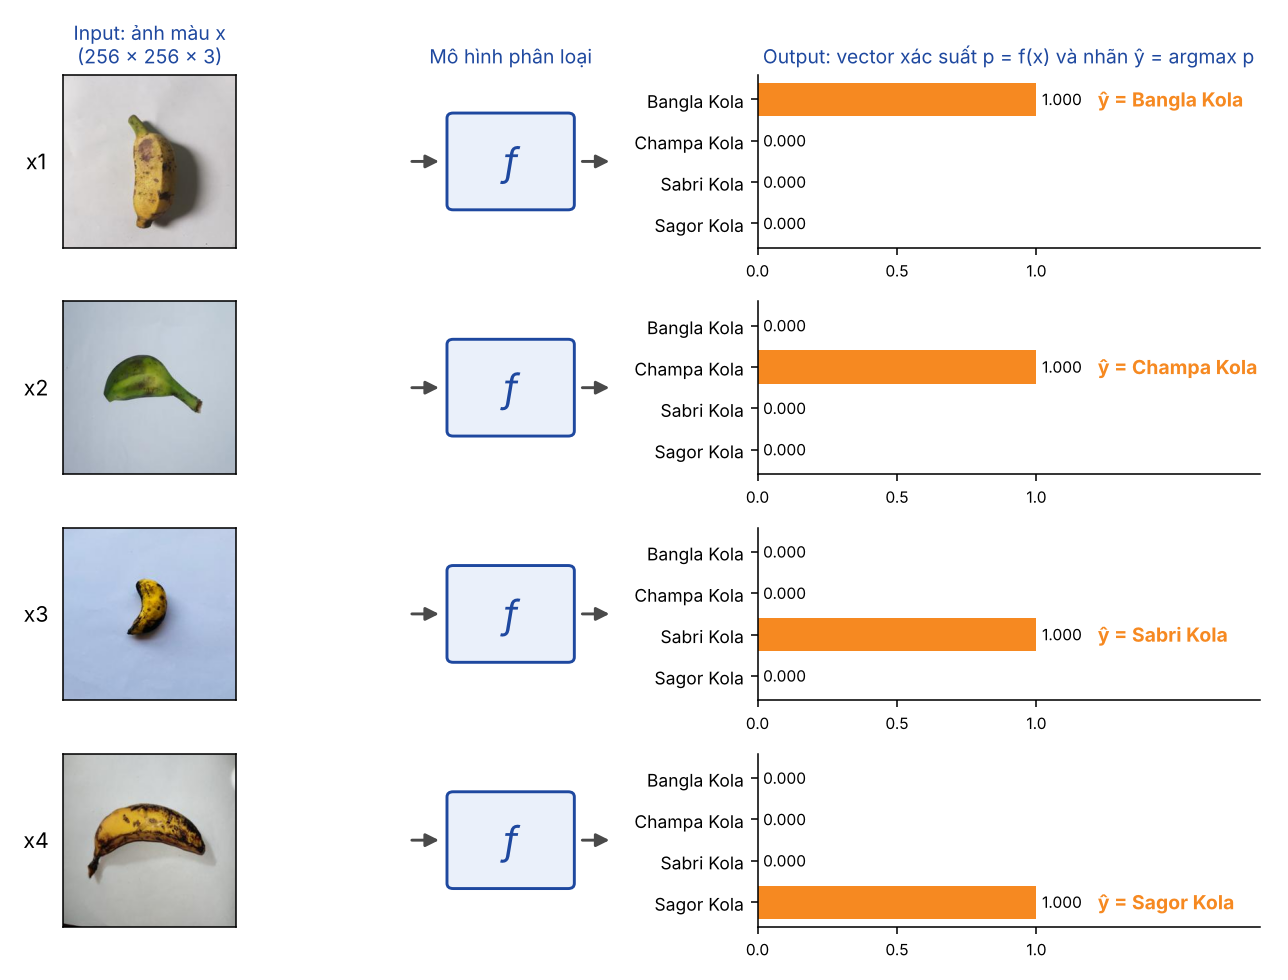
\includegraphics[width=\linewidth,height=0.74\textheight,keepaspectratio]{../results/figures/problem_io.png}\end{center}
\note{Đây là hình minh họa. Bên trái là bốn ảnh lấy từ tập test, mỗi ảnh một giống. Ảnh đi qua mô hình f. Bên phải là đầu ra: xác suất của bốn lớp, và nhãn dự đoán là lớp có cột cao nhất. Các xác suất trong hình là kết quả thật của mô hình MobileNetV3 trong đồ án.}
\end{frame}

\section{Phương pháp}
\begin{frame}{Tổng quan phương pháp}
\begin{center}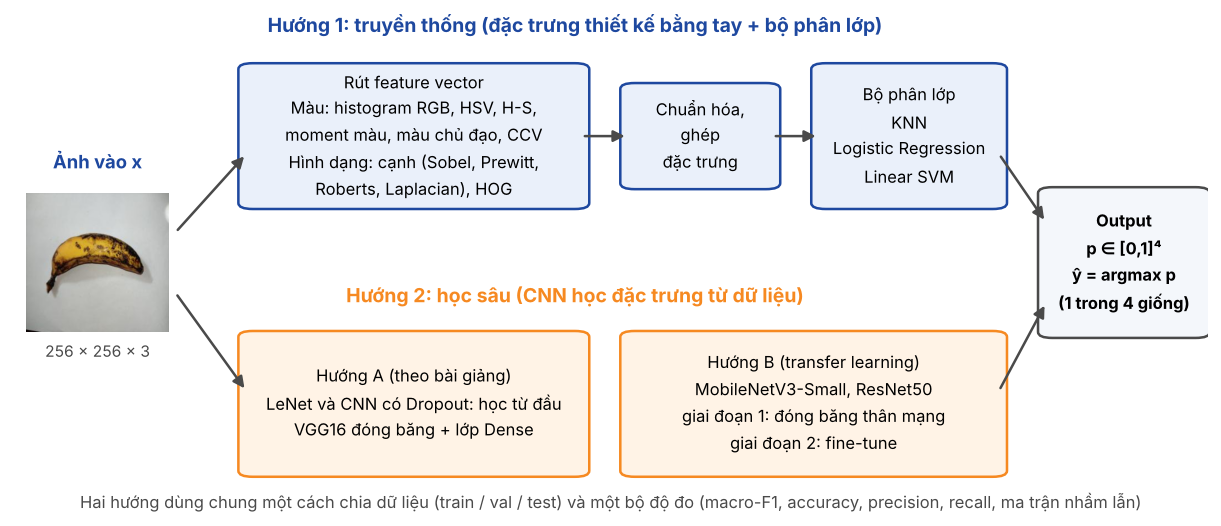
\includegraphics[width=\linewidth,height=0.56\textheight,keepaspectratio]{../results/figures/method_overview.png}\end{center}
\begin{itemize}\footnotesize
\item \textbf{Phần 1:} đặc trưng màu và KNN
\item \textbf{Phần 2:} cạnh, HOG, ghép đặc trưng, bộ phân lớp tuyến tính
\item \textbf{Phần 3:} CNN (hướng A theo bài giảng, hướng B fine-tune)
\item Cùng một cách chia dữ liệu và một bộ độ đo cho mọi phương pháp
\end{itemize}
\note{Nhóm em giải bài toán theo hai hướng. Hướng truyền thống: rút feature vector do con người thiết kế, gồm màu, cạnh và HOG, rồi đưa vào bộ phân lớp. Hướng học sâu: dùng CNN, mạng tự học đặc trưng từ dữ liệu. Phần phương pháp chia làm ba phần, mỗi bạn trình bày phần mình làm: phần một là đặc trưng màu và KNN, phần hai là cạnh, HOG, ghép đặc trưng và bộ phân lớp tuyến tính, phần ba là CNN. Các phương pháp này đều đã có sẵn, nên với mỗi phương pháp nhóm em chỉ nói ngắn gọn nó là gì, được đề xuất ở đâu, rồi nói rõ nhóm em dùng nó như thế nào.}
\end{frame}

\begin{frame}{Phần 1. Đặc trưng màu và KNN: là gì}
\begin{itemize}
\item \textbf{Histogram màu} (Swain và Ballard, 1991): tỉ lệ điểm ảnh rơi vào từng khoảng màu; không giữ vị trí điểm ảnh
\item \textbf{Moment màu} (Stricker và Orengo, 1995): trung bình, độ lệch chuẩn, độ lệch của từng kênh màu
\item \textbf{Color Coherence Vector, CCV} (Pass và cộng sự, 1996): với mỗi màu, tách điểm ảnh thuộc vùng liên thông lớn và điểm ảnh rời rạc
\item Đều là \textbf{feature vector toàn cục}: biết rõ ý nghĩa từng phần tử, mỗi phần tử tính từ toàn bộ ảnh
\item \textbf{KNN} (Cover và Hart, 1967): gán nhãn theo k ảnh huấn luyện gần nhất; không có bước huấn luyện
\end{itemize}
\vfill{\scriptsize\color{uitgray}Tài liệu: Color Indexing: \href{https://doi.org/10.1007/BF00130487}{\texttt{doi.org/10.1007/BF00130487}} \textbar{} Moment màu: \href{https://doi.org/10.1117/12.205308}{\texttt{doi.org/10.1117/12.205308}} \textbar{} CCV: \href{https://doi.org/10.1145/244130.244148}{\texttt{doi.org/10.1145/244130.244148}} \textbar{} KNN: \href{https://doi.org/10.1109/TIT.1967.1053964}{\texttt{doi.org/10.1109/TIT.1967.1053964}}}
\note{Em xin trình bày phần một: đặc trưng màu và KNN. Histogram màu đếm tỉ lệ điểm ảnh rơi vào từng khoảng màu, nó không quan tâm điểm ảnh nằm ở đâu. Moment màu tóm tắt phân bố màu của mỗi kênh bằng ba con số. CCV bổ sung cho histogram thông tin điểm ảnh có thuộc một vùng liên thông lớn hay không. Cả ba đều là feature vector toàn cục: mình hiểu ý nghĩa của từng phần tử, và mỗi phần tử được tính từ toàn bộ ảnh. Bộ phân lớp đi kèm là KNN: ảnh mới được gán nhãn theo k ảnh huấn luyện gần nó nhất. Tài liệu gốc của từng phương pháp nằm ở cuối slide.}
\end{frame}

\begin{frame}{Phần 1. Đặc trưng màu và KNN: nhóm dùng như thế nào}
\begin{columns}[T]
\begin{column}{0.36\textwidth}
\begin{itemize}\footnotesize
\item Histogram chia cho tổng số điểm ảnh (tổng bằng 1)
\item \textbf{Chuẩn hóa trước khi đo khoảng cách}: z-score từng chiều, hoặc đưa về vector đơn vị
\item KNN: khảo sát k, độ đo (Euclidean, Manhattan, cosine, Hellinger), cách bình chọn
\item Chọn bằng 5-fold cross-validation: \textbf{k = 1} tốt nhất
\end{itemize}
\end{column}
\begin{column}{0.62\textwidth}
\begin{center}\begin{adjustbox}{max width=\linewidth,max totalheight=0.74\textheight}
\rowcolors{2}{uitbg}{white}
\begin{tabular}{lll}\toprule
\textbf{Đặc trưng} & \textbf{Cách dùng trong đồ án} & \textbf{Số chiều} \\ \midrule
Histogram RGB & 32 bin mỗi kênh, ghép 3 kênh & 96 \\
Histogram HSV & (8, 8, 8) bin cho (H, S, V) & 512 \\
Histogram H-S & (8, 8) bin, bỏ kênh độ sáng V & 64 \\
Moment màu & 3 moment $\times$ 3 kênh HSV & 9 \\
Màu chủ đạo & k-means, k = 3: (tỉ lệ, R, G, B) mỗi cụm & 12 \\
CCV & 64 màu, vùng liên thông từ 1\% ảnh & 128 \\
\bottomrule\end{tabular}
\end{adjustbox}\end{center}
\end{column}
\end{columns}
\note{Đây là cách nhóm em dùng. Histogram RGB lấy 32 bin mỗi kênh, được 96 chiều. Histogram HSV lấy 8 bin mỗi kênh, được 512 chiều. Histogram H-S chỉ lấy hai kênh H và S, bỏ kênh độ sáng, được 64 chiều. Moment màu 9 chiều, màu chủ đạo 12 chiều, CCV 128 chiều. Trước khi đo khoảng cách, vector được chuẩn hóa. Lý do là hai vector cùng hướng nhưng khác độ lớn thì độ tương đồng là một trăm phần trăm, nhưng nếu không chuẩn hóa, khoảng cách Euclidean giữa chúng lại khác không. Với KNN, nhóm em khảo sát số láng giềng k, độ đo và cách bình chọn bằng 5-fold cross-validation, và k bằng 1 cho kết quả tốt nhất.}
\end{frame}

\begin{frame}{Phần 2. Cạnh, HOG và bộ phân lớp tuyến tính: là gì}
\begin{itemize}
\item \textbf{Toán tử cạnh}: Roberts, Prewitt, Sobel xấp xỉ đạo hàm bậc nhất; Laplacian xấp xỉ đạo hàm bậc hai
\item \textbf{HOG} (Dalal và Triggs, CVPR 2005): chia ảnh thành cell, mỗi cell một histogram hướng gradient, chuẩn hóa theo block; mô tả \textbf{hình dạng}
\item HOG là \textbf{feature vector cục bộ}: mỗi phần tử tính trên một cell, nên giữ được thông tin vị trí
\item \textbf{Logistic Regression, Linear SVM}: bộ phân lớp tuyến tính, học trọng số cho từng chiều của đặc trưng
\end{itemize}
\vfill{\scriptsize\color{uitgray}Tài liệu: HOG: \href{https://doi.org/10.1109/CVPR.2005.177}{\texttt{doi.org/10.1109/CVPR.2005.177}} \textbar{} SVM: \href{https://doi.org/10.1007/BF00994018}{\texttt{doi.org/10.1007/BF00994018}} \textbar{} scikit-learn: \href{https://scikit-learn.org}{\texttt{scikit-learn.org}}}
\note{Em xin trình bày phần hai. Đặc trưng màu không biết gì về hình dạng, nên nhóm em dùng thêm đặc trưng cạnh và HOG. Các toán tử Roberts, Prewitt, Sobel xấp xỉ đạo hàm bậc nhất của ảnh, Laplacian xấp xỉ đạo hàm bậc hai. HOG do Dalal và Triggs đề xuất năm 2005: ảnh được chia thành các cell, mỗi cell có một histogram của hướng gradient, rồi chuẩn hóa theo block. HOG mô tả hình dạng của vật. Khác với histogram màu, HOG là đặc trưng cục bộ: mỗi phần tử tính trên một cell, nên nó giữ thông tin vị trí. Bộ phân lớp ở phần này là Logistic Regression và Linear SVM, đều là bộ phân lớp tuyến tính.}
\end{frame}

\begin{frame}{Phần 2. Cạnh, HOG, ghép đặc trưng: nhóm dùng như thế nào}
\begin{columns}[T]
\begin{column}{0.50\textwidth}
\begin{itemize}\footnotesize
\item \textbf{HOG tự cài đặt theo bài giảng}: ảnh xám 64 $\times$ 128, cell 8 $\times$ 8, 9 bin, block 16 $\times$ 16 chuẩn hóa L2, được \textbf{3780 chiều}
\item Đối chiếu với scikit-image: lệch tối đa 2.2$\cdot$10$^{-7}$
\item \textbf{Vector cạnh}: tổng độ lớn gradient theo 256 hàng và 256 cột, 512 chiều
\item \textbf{Ghép màu với HOG}: chuẩn hóa z-score từng phần, chia cho căn số chiều để hai phần đóng góp ngang nhau
\item Cấu hình chốt bằng 5-fold CV: \textbf{Hist H-S + HOG + Logistic Regression (C = 100)}, 3844 chiều
\end{itemize}
\end{column}
\begin{column}{0.48\textwidth}
\begin{center}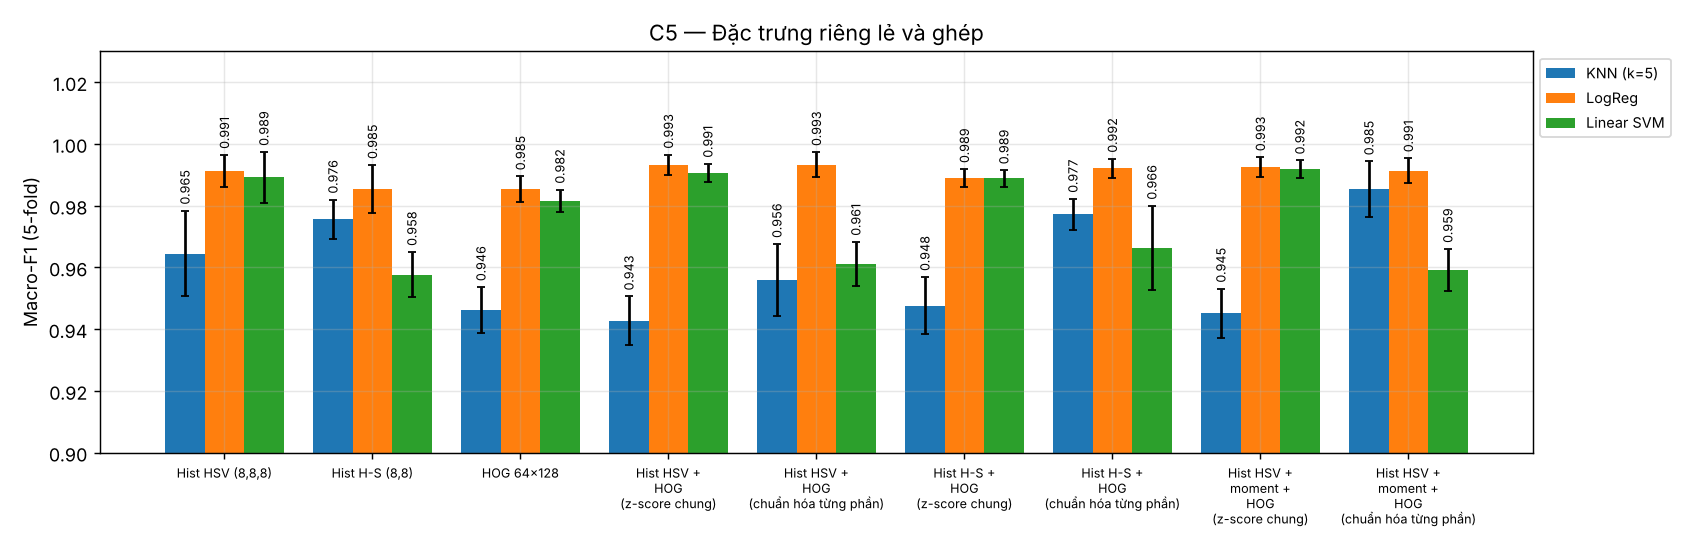
\includegraphics[width=\linewidth,height=0.72\textheight,keepaspectratio]{../results/figures/C5_fusion.png}\end{center}
\end{column}
\end{columns}
\note{Về cách dùng. HOG nhóm em tự cài đặt theo đúng các bước trong bài giảng: ảnh xám 64 nhân 128, cell 8 nhân 8, 9 bin, block 16 nhân 16 có chuẩn hóa L2, ra vector 3780 chiều. Nhóm em tự cài đặt để có thể bật tắt bước chuẩn hóa block trong thí nghiệm, và đã đối chiếu với thư viện scikit-image, hai kết quả gần như trùng nhau. Vector cạnh là tổng độ lớn gradient theo từng hàng và từng cột, 512 chiều. Điểm khác của nhóm em là cách ghép: phần màu chỉ có 64 chiều, phần HOG có 3780 chiều. Nếu ghép thẳng thì HOG lấn át. Nên mỗi phần được chuẩn hóa riêng rồi chia cho căn số chiều, để hai phần đóng góp ngang nhau. Hình bên phải cho thấy ghép theo cách này tốt hơn từng đặc trưng riêng lẻ. Cấu hình cuối cùng của hướng truyền thống là histogram H-S ghép HOG, phân lớp bằng Logistic Regression.}
\end{frame}

\begin{frame}{Phần 3. CNN hướng A (theo bài giảng): là gì}
\begin{itemize}
\item \textbf{LeNet-5} (LeCun và cộng sự, 1998): hai cặp lớp tích chập và lấy mẫu, sau đó là các lớp kết nối đầy đủ
\item \textbf{Dropout} (Srivastava và cộng sự, 2014): tắt ngẫu nhiên nơ-ron lúc huấn luyện để giảm quá khớp
\item \textbf{VGG16} (Simonyan và Zisserman, 2015): 13 lớp tích chập 3 $\times$ 3 và 3 lớp kết nối đầy đủ, huấn luyện trên ImageNet \textbf{1000 lớp}
\item \textbf{Transfer learning}: dùng lại phần tích chập đã học làm bộ rút đặc trưng
\item Đặc trưng do CNN sinh ra là \textbf{embedding}: không giải thích được ý nghĩa từng phần tử
\end{itemize}
\vfill{\scriptsize\color{uitgray}Tài liệu: LeNet: \href{https://doi.org/10.1109/5.726791}{\texttt{doi.org/10.1109/5.726791}} \textbar{} Dropout: \href{https://jmlr.org/papers/v15/srivastava14a.html}{\texttt{jmlr.org/papers/v15/srivastava14a.html}} \textbar{} VGG16: \href{https://arxiv.org/abs/1409.1556}{\texttt{arxiv.org/abs/1409.1556}}}
\note{Em xin trình bày phần ba, CNN. Hướng A là các mô hình đúng như ví dụ trong bài giảng. LeNet gồm hai cặp lớp tích chập và lấy mẫu, sau đó là các lớp kết nối đầy đủ. Dropout là kỹ thuật tắt ngẫu nhiên một số nơ-ron lúc huấn luyện để giảm quá khớp. VGG16 là mạng 16 lớp, được huấn luyện sẵn trên ImageNet với 1000 lớp. Transfer learning nghĩa là dùng lại phần tích chập đã học của VGG16 để rút đặc trưng cho bài toán của mình. Khác với feature vector ở hai phần trước, đặc trưng do CNN sinh ra gọi là embedding, mình không giải thích được ý nghĩa của từng phần tử.}
\end{frame}

\begin{frame}{Phần 3. CNN hướng A: nhóm dùng như thế nào}
\begin{center}\begin{adjustbox}{max width=\linewidth,max totalheight=0.74\textheight}
\rowcolors{2}{uitbg}{white}
\begin{tabular}{l >{\raggedright\arraybackslash}p{7.6cm} l >{\raggedright\arraybackslash}p{2.6cm}}\toprule
\textbf{Mô hình} & \textbf{Cách dùng trong đồ án} & \textbf{Ảnh vào} & \textbf{Số tham số} \\ \midrule
a\_lenet & Cấu trúc LeNet, đổi ảnh vào thành ảnh màu, lớp ra 4 lớp; huấn luyện từ đầu & 64 $\times$ 64 $\times$ 3 & 337976 \\
a\_dropout & Conv(32) $\rightarrow$ Conv(16) $\rightarrow$ Dense(128) $\rightarrow$ Dropout(0.5) $\rightarrow$ Dense(64) $\rightarrow$ Softmax(4); huấn luyện từ đầu & 128 $\times$ 128 $\times$ 3 & 1746260 \\
a\_vgg16 & Bỏ 3 lớp FC của VGG16, đóng băng phần tích chập (ra 7 $\times$ 7 $\times$ 512), thêm Flatten $\rightarrow$ Dense(1024) $\rightarrow$ Dense(256) $\rightarrow$ Softmax(4) & 224 $\times$ 224 $\times$ 3 & 40669252 (huấn luyện 25954564) \\
\bottomrule\end{tabular}
\end{adjustbox}\end{center}
\note{Nhóm em dùng như sau. Mô hình a\_lenet giữ cấu trúc LeNet, đổi ảnh vào thành ảnh màu 64 nhân 64 và lớp ra thành 4 lớp, huấn luyện từ đầu. Mô hình a\_dropout là CNN hai lớp tích chập, có Dropout 0.5, ảnh vào 128 nhân 128. Với VGG16: mạng gốc huấn luyện trên 1000 lớp, còn bài của nhóm em chỉ có 4 lớp. Nên nhóm em bỏ ba lớp kết nối đầy đủ ở cuối, giữ nguyên và đóng băng phần tích chập, rồi thêm phần đầu mới gồm Flatten, hai lớp Dense và lớp Softmax 4 lớp. Chỉ phần đầu mới được huấn luyện.}
\end{frame}

\begin{frame}{Phần 3. CNN hướng B (fine-tune): là gì}
\begin{itemize}
\item \textbf{MobileNetV3} (Howard và cộng sự, ICCV 2019): họ mạng thiết kế cho thiết bị di động, có hai phiên bản Large và Small
\item \textbf{ResNet} (He và cộng sự, CVPR 2016): dùng kết nối tắt để huấn luyện được mạng rất sâu
\item Cả hai có sẵn trọng số huấn luyện trên ImageNet (Keras Applications)
\item \textbf{Fine-tune}: không đóng băng hẳn, mà huấn luyện tiếp trọng số ImageNet trên dữ liệu mới với learning rate nhỏ
\end{itemize}
\vfill{\scriptsize\color{uitgray}Tài liệu: MobileNetV3: \href{https://arxiv.org/abs/1905.02244}{\texttt{arxiv.org/abs/1905.02244}} \textbar{} ResNet: \href{https://arxiv.org/abs/1512.03385}{\texttt{arxiv.org/abs/1512.03385}} \textbar{} Keras Applications: \href{https://keras.io/api/applications/}{\texttt{keras.io/api/applications/}}}
\note{Hướng B dùng mạng lớn hơn, huấn luyện sẵn trên ImageNet rồi fine-tune. MobileNetV3 là họ mạng thiết kế cho thiết bị di động, có hai phiên bản Large và Small. ResNet dùng kết nối tắt để huấn luyện được mạng rất sâu. Fine-tune khác với đóng băng ở chỗ mình huấn luyện tiếp cả phần thân trên dữ liệu của mình, với learning rate nhỏ. Chi tiết kiến trúc bên trong của hai mạng này có trong bài báo gốc ở cuối slide, nhóm em chỉ sử dụng chúng làm phần thân rút đặc trưng.}
\end{frame}

\begin{frame}{Phần 3. CNN hướng B: nhóm dùng như thế nào}
\begin{columns}[T]
\begin{column}{0.50\textwidth}
\begin{itemize}\footnotesize
\item Phiên bản: \textbf{MobileNetV3-Small} (embedding \textbf{576 chiều}) và \textbf{ResNet50} (2048 chiều), ảnh 224 $\times$ 224
\item Mạng gốc phân loại 1000 lớp, bài toán có 4 lớp: thay phần đầu bằng GlobalAveragePooling $\rightarrow$ Dropout(0.2) $\rightarrow$ Softmax(4)
\item \textbf{Giai đoạn 1:} đóng băng phần thân, chỉ huấn luyện lớp Softmax
\item \textbf{Giai đoạn 2:} mở băng (toàn mạng với MobileNetV3, khối conv5 với ResNet50), learning rate 1e-4 và 1e-5, có tăng cường ảnh
\item Giữ BatchNorm đóng băng khi fine-tune; Adam, cross-entropy, dừng sớm theo macro-F1 trên val
\end{itemize}
\end{column}
\begin{column}{0.48\textwidth}
\begin{center}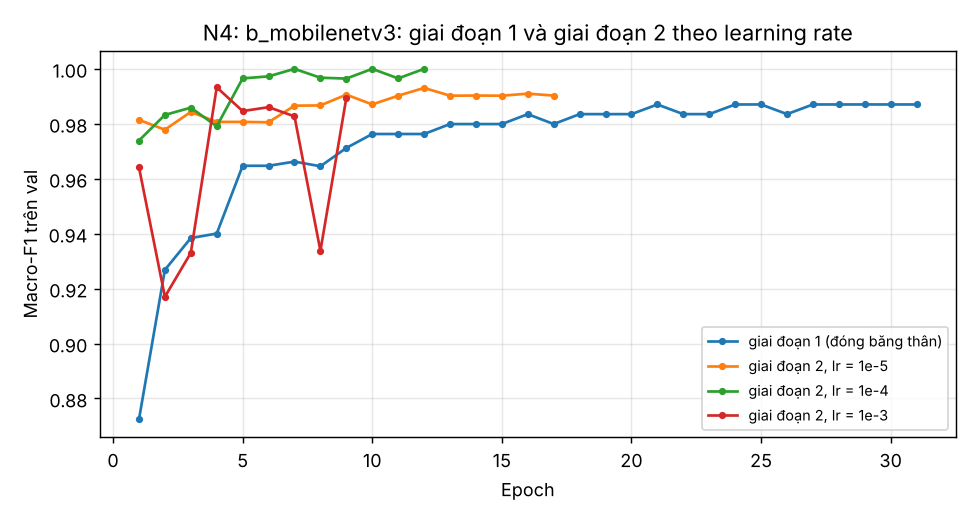
\includegraphics[width=\linewidth,height=0.72\textheight,keepaspectratio]{../results/figures/N4_finetune_lr.png}\end{center}
\end{column}
\end{columns}
\note{Nhóm em dùng phiên bản MobileNetV3-Small, embedding sau lớp GlobalAveragePooling có 576 chiều, và ResNet50 với embedding 2048 chiều. Ảnh vào 224 nhân 224. Mạng gốc phân loại 1000 lớp, nên nhóm em thay phần đầu bằng lớp Softmax 4 lớp. Huấn luyện gồm hai giai đoạn. Giai đoạn một đóng băng phần thân, chỉ huấn luyện lớp Softmax mới. Giai đoạn hai mở băng phần thân và huấn luyện tiếp với learning rate nhỏ, có tăng cường ảnh như lật, xoay, phóng to thu nhỏ. Một chi tiết nhóm em rút ra khi làm: khi fine-tune phải giữ các lớp BatchNorm đóng băng. Lần đầu nhóm em để mở, accuracy trên train tụt xuống còn khoảng 0.36. Hình bên phải là macro-F1 trên val theo epoch của giai đoạn một và giai đoạn hai với các learning rate khác nhau.}
\end{frame}

\begin{frame}{Điểm khác biệt giữa các phương pháp}
\begin{center}\begin{adjustbox}{max width=\linewidth,max totalheight=0.74\textheight}
\rowcolors{2}{uitbg}{white}
\begin{tabular}{>{\raggedright\arraybackslash}p{3.6cm} >{\raggedright\arraybackslash}p{1.7cm} >{\raggedright\arraybackslash}p{2.4cm} >{\raggedright\arraybackslash}p{1.4cm} >{\raggedright\arraybackslash}p{1.3cm} >{\raggedright\arraybackslash}p{2.4cm}}\toprule
\textbf{Phương pháp} & \textbf{Loại biểu diễn} & \textbf{Toàn cục hay cục bộ} & \textbf{Số chiều} & \textbf{Giữ vị trí} & \textbf{Học đặc trưng từ dữ liệu} \\ \midrule
Histogram màu, moment màu & feature vector & toàn cục & 9 đến 512 & không & không \\
Vector cạnh, HOG & feature vector & cục bộ (hàng, cột, cell) & 512, 3780 & có & không \\
CNN học từ đầu (LeNet) & embedding & cục bộ (cửa sổ tích chập) & 84 & có & có, cần nhiều dữ liệu \\
CNN ImageNet đóng băng (VGG16) & embedding & cục bộ (cửa sổ tích chập) & 7 $\times$ 7 $\times$ 512 & có & chỉ phần đầu mới \\
CNN ImageNet fine-tune (MobileNetV3) & embedding & cục bộ (cửa sổ tích chập) & 576 & mất sau GAP & có, chỉnh từ ImageNet \\
\bottomrule\end{tabular}
\end{adjustbox}\end{center}
\note{Bảng này tóm tắt điểm khác biệt giữa các phương pháp. Histogram và moment màu là feature vector toàn cục, ít chiều, không giữ vị trí. HOG và vector cạnh là feature vector cục bộ, giữ được vị trí. Ba dòng cuối là embedding của CNN: mỗi giá trị tính trên một cửa sổ tích chập nên cũng là cục bộ. Khác nhau ở chỗ có học đặc trưng từ dữ liệu hay không: LeNet học từ đầu nên cần nhiều dữ liệu, VGG16 đóng băng thì không học lại, MobileNetV3 fine-tune thì chỉnh lại từ trọng số ImageNet. Từ bảng này nhóm em đặt ra các dự đoán và kiểm chứng ở phần thực nghiệm.}
\end{frame}

\section{Thực nghiệm}
\begin{frame}{Dataset}
\begin{columns}[T]
\begin{column}{0.46\textwidth}
\begin{itemize}\footnotesize
\item \textbf{BananaImageBD}, Version 2 (Mendeley Data, CC BY 4.0), dataset có sẵn của Ferdaus và cộng sự
\item \textbf{2471 ảnh} gốc, 256 $\times$ 256, 4 giống: Champa 994, Sagor 524, Sabri 509, Bangla 444
\item Mỗi quả đặt trên giấy trắng, chụp bằng điện thoại từ bốn mặt
\item Chia cố định, giữ tỉ lệ lớp: \textbf{train 1729, val 371, test 371}
\item Tập test chỉ dùng một lần ở cuối
\end{itemize}
\end{column}
\begin{column}{0.52\textwidth}
\begin{center}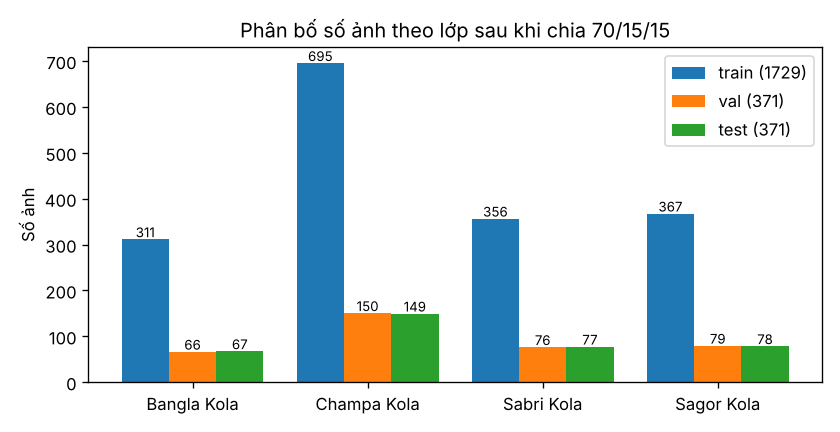
\includegraphics[width=\linewidth,height=0.72\textheight,keepaspectratio]{../results/figures/data_split_counts.png}\end{center}
\end{column}
\end{columns}
\vfill{\scriptsize\color{uitgray}Tài liệu: Dataset: \href{https://data.mendeley.com/datasets/ptfscwtnyz/2}{\texttt{data.mendeley.com/datasets/ptfscwtnyz/2}} \textbar{} Bài báo mô tả: \href{https://doi.org/10.1016/j.dib.2024.111239}{\texttt{doi.org/10.1016/j.dib.2024.111239}}}
\note{Về dataset. Nhóm em dùng bộ BananaImageBD, là bộ dữ liệu có sẵn, công bố trên Mendeley Data. Có 2471 ảnh gốc kích thước 256 nhân 256 của bốn giống, trong đó Champa Kola nhiều nhất với 994 ảnh và Bangla Kola ít nhất với 444 ảnh. Nhóm em chia cố định thành train, val và test theo tỉ lệ 70, 15, 15, giữ nguyên tỉ lệ các lớp. Tập test chỉ dùng một lần ở cuối.}
\end{frame}

\begin{frame}{Độ đo đánh giá}
Với mỗi lớp $c$ (coi $c$ là dương, 3 lớp còn lại là âm):
\[ \text{Precision}_c=\frac{TP}{TP+FP},\qquad \text{Recall}_c=\frac{TP}{TP+FN},\qquad F1_c=\frac{2\cdot \text{Precision}_c\cdot \text{Recall}_c}{\text{Precision}_c+\text{Recall}_c} \]
\[ \text{Accuracy}=\frac{\text{số ảnh đoán đúng}}{\text{tổng số ảnh}},\qquad \textbf{Macro-F1}=\frac{1}{4}\sum_{c=1}^{4}F1_c \]
\begin{itemize}
\item \textbf{Macro-F1 là chỉ số chính}: dữ liệu lệch lớp (994 so với 444 ảnh), mỗi lớp được tính trọng số như nhau
\item \textbf{Ma trận nhầm lẫn}: hàng là lớp thật, cột là lớp dự đoán. Chia theo tổng hàng thì đường chéo là recall
\item Ví dụ (\texttt{a\_vgg16}, test): hàng Bangla Kola có 67 ảnh, $65/67=0.970$ đoán đúng, $2/67=0.030$ bị nhầm thành Sagor Kola
\item Kết quả cuối kèm khoảng tin cậy 95\% (bootstrap); truyền thống chọn tham số bằng 5-fold cross-validation
\end{itemize}
\note{Nhóm em sử dụng các độ đo cơ bản của bài toán phân loại đã học trong môn học: accuracy, precision, recall, F1 và ma trận nhầm lẫn. Chỉ số chính là macro-F1, vì dữ liệu lệch lớp.}
\end{frame}

\begin{frame}{Kết quả trên tập test (371 ảnh)}
\begin{center}\begin{adjustbox}{max width=\linewidth,max totalheight=0.74\textheight}
\rowcolors{2}{uitbg}{white}
\begin{tabular}{>{\raggedright\arraybackslash}p{2.7cm} >{\raggedright\arraybackslash}p{5.6cm} l l l}\toprule
\textbf{Nhóm} & \textbf{Mô hình} & \textbf{Macro-F1 test} & \textbf{KTC 95\% (bootstrap)} & \textbf{Số ảnh sai / 371} \\ \midrule
Truyền thống (màu) & Hist HSV (8,8,8) + LogReg C=0.1 & 0.994 & [0.984; 1.000] & 2 \\
Truyền thống (cạnh) & Cạnh Roberts + KNN k=1, Manhattan, ưu tiên điểm gần & 0.964 & [0.944; 0.982] & 12 \\
Truyền thống (HOG) & HOG 64$\times$128 + LogReg C=0.1 & 0.990 & [0.977; 1.000] & 3 \\
Truyền thống (ghép) & Hist H-S + HOG + LogReg C=100, chuẩn hóa từng phần & 1.000 & [1.000; 1.000] & 0 \\
CNN hướng A & a\_lenet (biến thể: a\_lenet) & 0.978 & [0.960; 0.993] & 7 \\
CNN hướng A & a\_dropout (biến thể: a\_dropout\_aug) & 0.942 & [0.917; 0.965] & 21 \\
CNN hướng A & a\_vgg16 (biến thể: a\_vgg16\_lr1e-3) & 0.986 & [0.971; 0.997] & 4 \\
CNN hướng B & b\_mobilenetv3 (biến thể: b\_mobilenetv3\_lr1e-4) & 1.000 & [1.000; 1.000] & 0 \\
CNN hướng B & b\_resnet50 (biến thể: b\_resnet50) & 0.997 & [0.988; 1.000] & 1 \\
\bottomrule\end{tabular}
\end{adjustbox}\end{center}
\note{Đây là kết quả cuối trên tập test 371 ảnh. Hướng truyền thống tốt nhất là histogram H-S ghép HOG với Logistic Regression, macro-F1 1.000, đúng cả 371 ảnh. CNN hướng B với MobileNetV3 cũng đạt 1.000, đúng cả 371 ảnh. Trong hướng A, VGG16 đóng băng tốt nhất với 0.986, còn LeNet huấn luyện từ đầu đạt 0.978. Khoảng tin cậy của các mô hình dẫn đầu chồng lên nhau, nên nhóm em không kết luận mô hình nào hơn mô hình nào trong nhóm này.}
\end{frame}

\begin{frame}{Kết quả: màu hay hình dạng?}
\begin{columns}[T]
\begin{column}{0.42\textwidth}
\begin{itemize}\footnotesize
\item Xáo trộn ảnh thành lưới 4 $\times$ 4: histogram không đổi (sụt 0.000), HOG rơi về mức đoán mò
\item Chuyển sang ảnh xám: đặc trưng màu sụt 0.04 đến 0.23, \textbf{HOG vẫn đạt 0.986}
\item Bốn giống phân biệt được bằng \textbf{cả màu} (Hist HSV 0.991) \textbf{lẫn hình dạng} (HOG 0.986)
\item Ghép màu với HOG tốt nhất: 0.996 $\pm$ 0.003 (5-fold)
\end{itemize}
\end{column}
\begin{column}{0.56\textwidth}
\begin{center}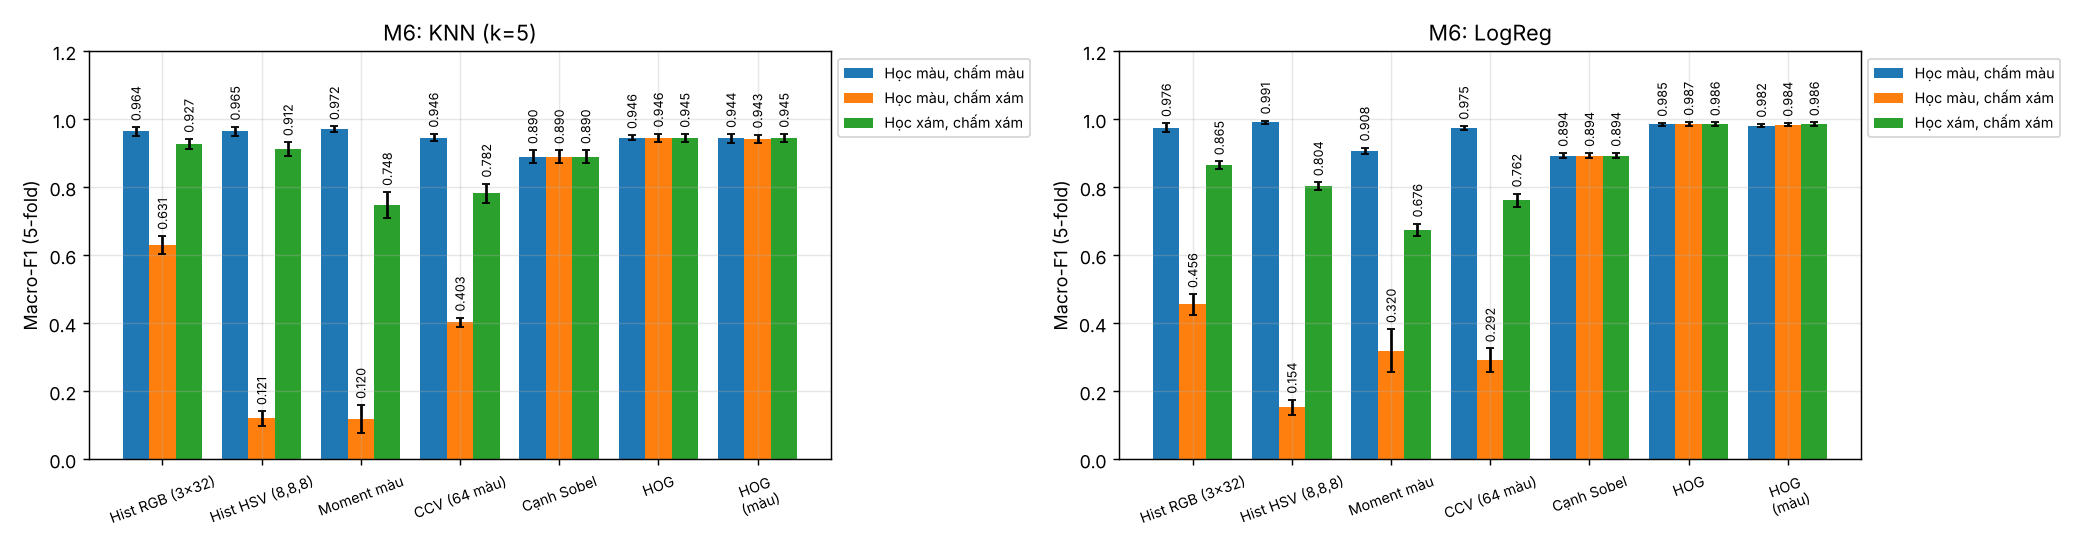
\includegraphics[width=\linewidth,height=0.72\textheight,keepaspectratio]{../results/figures/M6_grayscale.png}\end{center}
\end{column}
\end{columns}
\note{Một số kết quả kiểm chứng tính chất của đặc trưng. Khi xáo trộn ảnh thành lưới 4 nhân 4, histogram màu không đổi một chút nào, vì nó không giữ vị trí, còn HOG thì rơi về mức đoán mò. Khi chuyển ảnh sang xám, đặc trưng màu sụt, còn HOG vẫn đạt 0.986. Vậy bốn giống chuối phân biệt được bằng cả màu lẫn hình dạng, và ghép hai loại lại cho kết quả tốt nhất.}
\end{frame}

\begin{frame}{Kết quả: CNN và lượng dữ liệu}
\begin{columns}[T]
\begin{column}{0.46\textwidth}
\begin{itemize}\footnotesize
\item Chỉ 25\% dữ liệu train: mô hình có trọng số ImageNet (0.967, 0.975) đã ngang LeNet dùng đủ dữ liệu (0.973)
\item \textbf{MobileNetV3-Small}: 0.94 triệu tham số, file \textbf{4.3 MB}, 12.5 ms mỗi ảnh trên CPU
\item a\_vgg16: 40.7 triệu tham số, file 163 MB, 130 ms mỗi ảnh
\item Trái dự đoán: Dropout không giúp ở a\_dropout (0.941 so với 0.953 khi bỏ Dropout, 3 seed)
\end{itemize}
\end{column}
\begin{column}{0.52\textwidth}
\begin{center}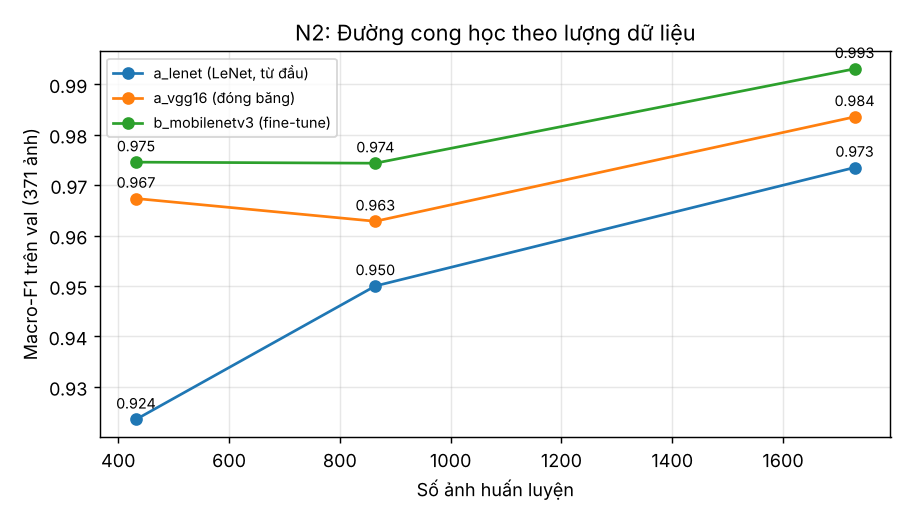
\includegraphics[width=\linewidth,height=0.72\textheight,keepaspectratio]{../results/figures/N2_learning_curve.png}\end{center}
\end{column}
\end{columns}
\note{Với CNN, hình bên phải là macro-F1 theo lượng dữ liệu huấn luyện. Chỉ với 25 phần trăm dữ liệu, hai mô hình dùng trọng số ImageNet đã ngang LeNet dùng toàn bộ dữ liệu. Đây là lợi ích của transfer learning khi dữ liệu ít. MobileNetV3-Small vừa chính xác nhất vừa nhẹ: file chỉ 4.3 megabyte và dự đoán 12.5 mili giây mỗi ảnh trên CPU, trong khi VGG16 nặng 163 megabyte. Cũng có kết quả trái dự đoán: Dropout không giúp ở mô hình a\_dropout. Nhóm em giải thích là 99 phần trăm tham số nằm ở lớp Dense đứng trước lớp Dropout, nên Dropout không chặn được quá khớp ở đó.}
\end{frame}

\begin{frame}{Khác tài liệu tham khảo (1): mô hình nhìn quả hay nhìn nền?}
\begin{columns}[T]
\begin{column}{0.44\textwidth}
\begin{itemize}\footnotesize
\item Dùng phân đoạn (Otsu, k-means) tách ảnh thành "chỉ quả" và "chỉ nền"
\item Chỉ dùng 4 góc ảnh (gần như không có chuối): HOG vẫn đạt 0.968, histogram màu 0.939
\item CNN dự đoán trên ảnh đã xóa quả chuối: 0.683 đến 0.792 (đoán mò khoảng 0.25)
\item \textbf{Dữ liệu thiên lệch theo bối cảnh chụp}: mỗi giống có nền và cỡ quả riêng
\item Chỉ nhìn quả: truyền thống 0.958, CNN 0.926 đến 0.952
\end{itemize}
\end{column}
\begin{column}{0.54\textwidth}
\begin{center}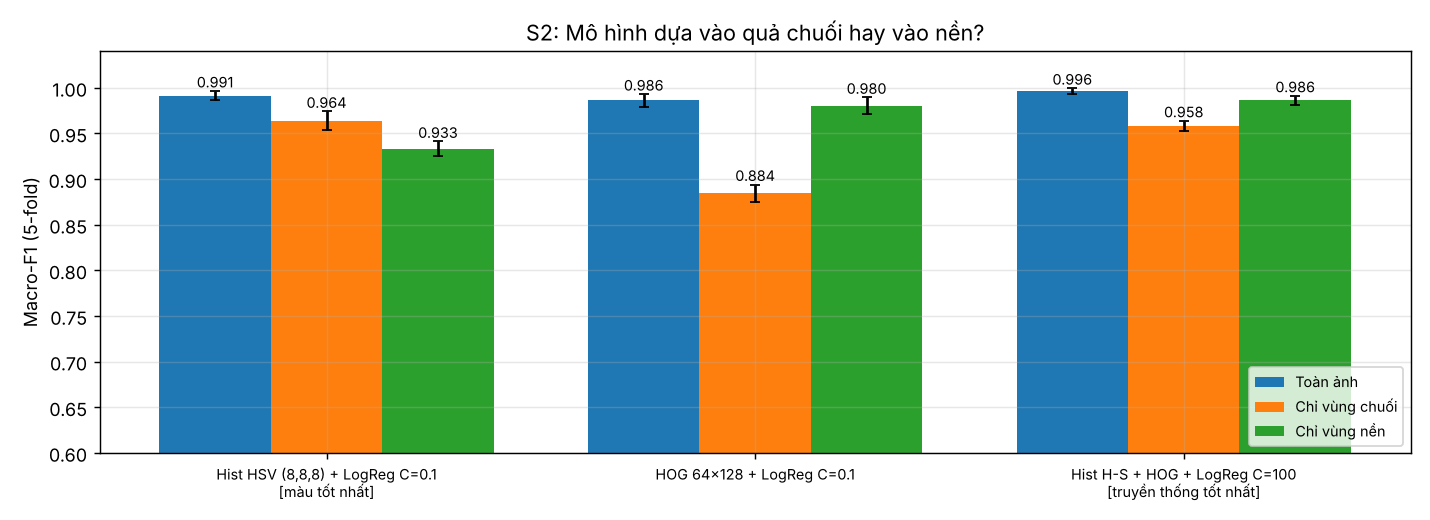
\includegraphics[width=\linewidth,height=0.72\textheight,keepaspectratio]{../results/figures/S2_background_bias.png}\end{center}
\end{column}
\end{columns}
\note{Phần này là thực nghiệm nhóm em tự thiết kế, không có trong tài liệu tham khảo. Kết quả gần 100 phần trăm làm nhóm em nghi ngờ: mô hình đang nhìn quả chuối hay nhìn nền? Nhóm em dùng các phương pháp phân đoạn đã học để tách ảnh thành phần chỉ có quả và phần chỉ có nền. Kết quả là chỉ dùng bốn góc ảnh, nơi gần như không có chuối, HOG vẫn đạt 0.968. CNN dự đoán trên ảnh đã xóa quả chuối vẫn đạt khoảng 0.7 đến 0.8, trong khi đoán mò chỉ là 0.25. Nghĩa là bộ dữ liệu có thiên lệch theo bối cảnh chụp: mỗi giống được chụp với nền và cỡ quả riêng, và mô hình học được cả điều đó. Đây là hạn chế quan trọng nhất mà nhóm em tìm ra.}
\end{frame}

\begin{frame}{Khác tài liệu tham khảo (2): bộ kiểm tra khó, đối chiếu bài báo}
\begin{itemize}\footnotesize
\item \textbf{Bộ kiểm tra khó}: 6 phép biến đổi trên tập test (thay nền, tối, sáng, nhiễu, xoay, che)
\item Thay nền: MobileNetV3 từ 1.000 xuống \textbf{0.794}; thêm ảnh train có nền thay ngẫu nhiên (X-b): \textbf{0.975}
\item Chạy lại phương pháp của bài báo (ViT + SVM): \textbf{99.49\%}, bài báo công bố 99.70\%
\item Cách chia fold của bài báo có rò rỉ: cao hơn chia đúng ở 19/19 tổ hợp (+0.11 đến +0.90 điểm)
\end{itemize}
\begin{center}\begin{adjustbox}{max width=\linewidth,max totalheight=0.40\textheight}
\rowcolors{2}{uitbg}{white}
\begin{tabular}{>{\raggedright\arraybackslash}p{5.4cm} >{\raggedright\arraybackslash}p{3.4cm} l l l l}\toprule
\textbf{Nhánh} & \textbf{Cấu hình đại diện} & \textbf{Ảnh gốc} & \textbf{Nền hoán đổi} & \textbf{Che 25\%} & \textbf{Điểm bền} \\ \midrule
G: pipeline gốc & b\_mobilenetv3 & 1.000 & 0.794 & 0.659 & 0.875 \\
X-a: xử lý dữ liệu, tiền xử lý lúc suy luận & b\_mobilenetv3 & 0.995 & 0.995 & 0.450 & 0.881 \\
X-b: xử lý dữ liệu, tăng cường có thay nền & b\_mobilenetv3 & 1.000 & 0.975 & 0.441 & 0.883 \\
T: Augmented của tác giả (không rò rỉ) & b\_mobilenetv3 & 0.998 & 0.867 & 0.736 & 0.909 \\
B1: bài báo, trong phạm vi môn học (CNN + bộ phân lớp) & MobileNetV3-Small + SVM tuyến tính & 0.993 & 0.742 & 0.575 & 0.836 \\
B2: bài báo, đúng phương pháp (ViT + SVM) & ViT-B/16 + SVM & 0.997 & 0.857 & 0.728 & 0.919 \\
\bottomrule\end{tabular}
\end{adjustbox}\end{center}
\note{Vì trên ảnh gốc hai mô hình đã đúng hết, nhóm em tạo thêm bộ kiểm tra khó gồm sáu phép biến đổi trên tập test, trong đó có phép thay nền: ghép quả chuối lên nền của ảnh thuộc lớp khác. Với phép thay nền, MobileNetV3 giảm từ 1.000 xuống 0.794. Khi nhóm em thêm vào tập train các ảnh có nền thay ngẫu nhiên, con số này lên lại 0.975. Nhóm em cũng chạy lại phương pháp của bài báo đã công bố trên bộ dữ liệu này, là Vision Transformer kết hợp SVM, và đạt 99.49 phần trăm, gần với 99.70 phần trăm bài báo công bố. Tuy nhiên cách chia fold của bài báo để ảnh gốc và bản tăng cường của nó nằm ở cả hai phía, nên kết quả cao hơn cách chia đúng ở cả 19 trên 19 tổ hợp nhóm em thử. Vision Transformer nằm ngoài nội dung môn học, nhóm em chỉ dùng để đối chiếu.}
\end{frame}

\begin{frame}{Chương trình demo}
\begin{columns}[T]
\begin{column}{0.36\textwidth}
\begin{itemize}\footnotesize
\item Viết bằng Gradio, chạy: python app/app.py
\item Dự đoán một ảnh: giống, xác suất 4 lớp, thời gian
\item So sánh 4 mô hình trên cùng một ảnh
\item Grad-CAM: vùng ảnh mà CNN dựa vào
\item Thử độ bền: đổi sáng, nhiễu, xoay, che, thay nền
\item Tính lại accuracy, precision, recall, F1, ma trận nhầm lẫn trên val và test
\end{itemize}
\end{column}
\begin{column}{0.62\textwidth}
\begin{center}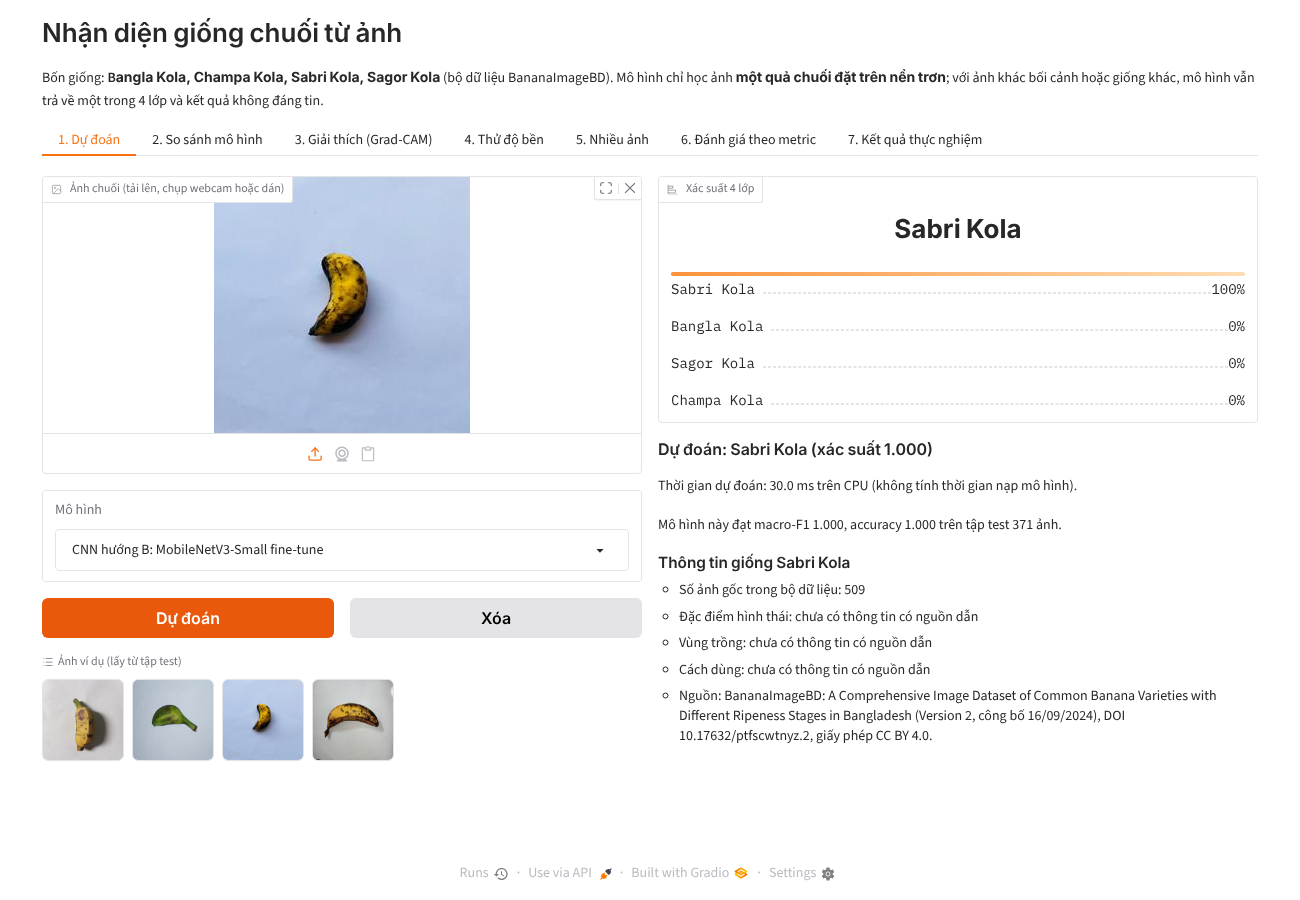
\includegraphics[width=\linewidth,height=0.72\textheight,keepaspectratio]{../results/figures/demo_screenshot.png}\end{center}
\end{column}
\end{columns}
\note{Nhóm em xin chạy chương trình demo. Chương trình viết bằng Gradio. (Chuyển sang cửa sổ demo, làm theo kịch bản demo trong file kịch bản.)}
\end{frame}

\section{Kết luận}
\begin{frame}{Nhận xét}
\begin{itemize}\small
\item \textbf{Ưu điểm}
\begin{itemize}
\item Hai mô hình đúng 371/371 ảnh test; MobileNetV3-Small chỉ 4.3 MB, 12.5 ms mỗi ảnh
\item So sánh mọi phương pháp trên cùng quy trình: test dùng một lần, cross-validation, khoảng tin cậy
\item 30 thí nghiệm kiểm chứng tính chất của phương pháp, ghi cả kết quả trái dự đoán
\item Chạy lại được toàn bộ bằng một lệnh; có demo
\end{itemize}
\item \textbf{Hạn chế}
\begin{itemize}
\item Dữ liệu thiên lệch theo nền: chỉ nhìn nền vẫn đạt 0.93 đến 0.99, nên kết quả 100\% chỉ đúng trên bộ dữ liệu này
\item Mỗi quả chụp bốn mặt, chia ngẫu nhiên không tách theo quả: kết quả lạc quan hơn 0.02 đến 0.07
\item Chưa có ảnh chụp thật ngoài bộ dữ liệu; chương trình không từ chối được ảnh ngoài 4 giống
\end{itemize}
\end{itemize}
\note{Về nhận xét. Ưu điểm: có hai mô hình đúng toàn bộ 371 ảnh test, trong đó MobileNetV3 rất nhẹ. Nhóm em so sánh mọi phương pháp trên cùng một quy trình đánh giá, và kiểm chứng tính chất của từng phương pháp bằng 30 thí nghiệm, ghi lại cả những kết quả trái dự đoán. Hạn chế: thứ nhất, dữ liệu thiên lệch theo nền, nên con số 100 phần trăm chỉ đúng trên bộ dữ liệu này, chưa chắc đúng với ảnh chụp ở nơi khác. Thứ hai, mỗi quả được chụp bốn mặt mà khi chia ngẫu nhiên thì ảnh của cùng một quả có thể nằm ở cả train và test, nên kết quả lạc quan hơn thực tế. Thứ ba, nhóm em chưa có ảnh chụp thật ngoài bộ dữ liệu để đánh giá, và chương trình chưa từ chối được ảnh ngoài bốn giống.}
\end{frame}

\begin{frame}{Kết luận}
\begin{itemize}
\item Đã xây dựng chương trình nhận diện 4 giống chuối; hai hướng đều đạt macro-F1 1.000 trên tập test
\item Phương pháp tốt khi tính chất của nó khớp với dữ liệu: histogram không biết vị trí, HOG không biết màu, CNN học từ đầu cần nhiều dữ liệu
\item Cách đánh giá quan trọng không kém mô hình: tăng cường trước khi chia tập làm kết quả đẹp hơn thực tế
\item Độ chính xác cao chưa chắc mô hình đã học đúng thứ cần học: ở đây mô hình dựa một phần vào nền
\item \textbf{Hướng phát triển:} ảnh ở bối cảnh khác, chia dữ liệu theo quả, thêm lớp "không thuộc 4 giống"
\end{itemize}
\note{Kết luận. Nhóm em đã xây dựng được chương trình nhận diện bốn giống chuối, cả hướng truyền thống lẫn hướng học sâu đều đạt macro-F1 bằng 1 trên tập test. Nhóm em rút ra ba điều: phương pháp tốt khi tính chất của nó khớp với dữ liệu, cách đánh giá quan trọng không kém mô hình, và độ chính xác cao chưa chắc mô hình đã học đúng thứ cần học. Nhóm em đã rất cố gắng và dành nhiều thời gian cho đồ án này. Tuy nhiên vẫn còn những phần chưa đạt như mong muốn, như chưa đánh giá được trên ảnh chụp thật ngoài bộ dữ liệu và chưa xử lý được ảnh ngoài phạm vi bốn giống. Đó cũng là hướng phát triển tiếp theo.}
\end{frame}

\begin{frame}{Tài liệu tham khảo}
\begin{itemize}\small
\item [1] Ferdaus và cộng sự (2024). BananaImageBD, Version 2. Mendeley Data. DOI 10.17632/ptfscwtnyz.2 (CC BY 4.0); bài báo mô tả: Data in Brief 58, 111239 (2025)
\item [2] Bài giảng môn CS231, Nhập môn Thị giác máy tính, Trường ĐH Công nghệ Thông tin
\item [3] Ergün (2025). High precision banana variety identification using vision transformer based feature extraction and SVM. Scientific Reports 15, 10366
\item [4] Swain, Ballard (1991), Color Indexing; Stricker, Orengo (1995); Pass, Zabih, Miller (1996), CCV; Dalal, Triggs (2005), HOG; Otsu (1979); Cover, Hart (1967), KNN
\item [5] LeCun và cộng sự (1998), LeNet; Simonyan, Zisserman (2015), VGG; He và cộng sự (2016), ResNet; Howard và cộng sự (2019), MobileNetV3
\item [6] Srivastava và cộng sự (2014), Dropout; Ioffe, Szegedy (2015), BatchNorm; Kingma, Ba (2015), Adam; Selvaraju và cộng sự (2017), Grad-CAM; Dosovitskiy và cộng sự (2021), ViT
\item [7] Thư viện: scikit-learn, scikit-image, OpenCV, TensorFlow và Keras, Gradio
\item Danh sách đầy đủ (40 tài liệu) và nguồn của từng hình ở mục 7 của báo cáo
\end{itemize}
\note{Đây là các tài liệu tham khảo chính. Danh sách đầy đủ nằm trong báo cáo.}
\end{frame}

\begin{frame}{Cảm ơn thầy và các bạn đã lắng nghe}
\begin{itemize}
\item Nhóm xin nhận câu hỏi và góp ý
\item Mã nguồn, báo cáo, slide và demo: github.com/Rod-HD/banana-classification
\end{itemize}
\note{Phần trình bày của nhóm em đến đây là hết. Em cảm ơn thầy và các bạn đã lắng nghe. Nhóm em xin nhận câu hỏi và góp ý ạ.}
\end{frame}

\appendix
\begin{frame}{Phụ lục. D1: Rò rỉ khi tăng cường ảnh trước khi chia}
\begin{columns}[T]
\begin{column}{0.36\textwidth}
\begin{itemize}\footnotesize
\item Histogram HSV + KNN: thổi phồng +0.021
\item HOG: $\approx$ 0 (trái dự đoán)
\item Rò rỉ chỉ hại khi đặc trưng bất biến với phép tăng cường
\end{itemize}
\end{column}
\begin{column}{0.62\textwidth}
\begin{center}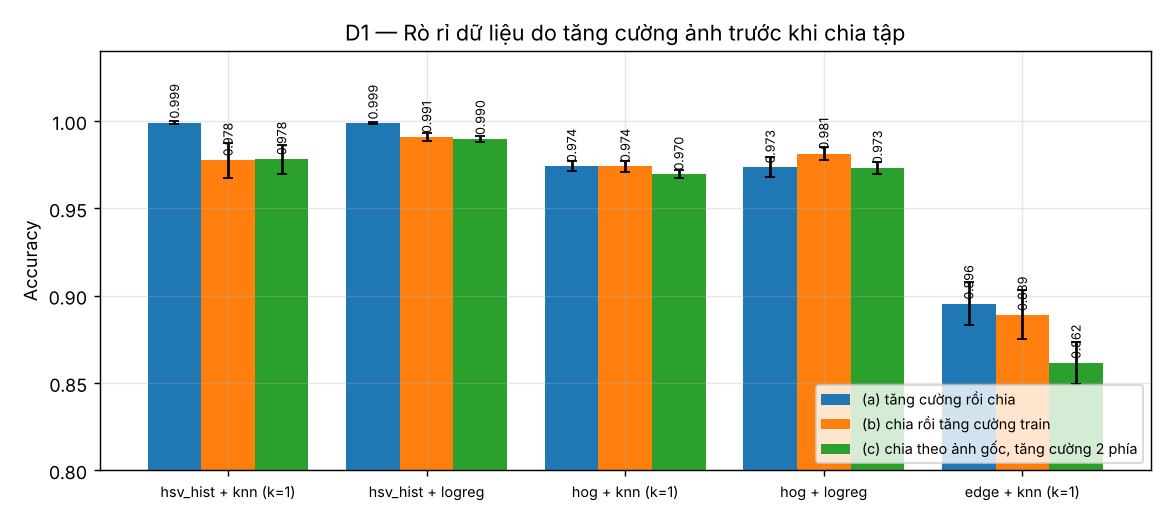
\includegraphics[width=\linewidth,height=0.72\textheight,keepaspectratio]{../results/figures/D1_leakage.png}\end{center}
\end{column}
\end{columns}
\note{Dự đoán: tăng cường rồi mới chia làm bản sao của ảnh test nằm trong train nên kết quả bị thổi phồng. Đúng với histogram vì histogram gần như không đổi khi lật/xoay. Với HOG mức thổi phồng gần 0 vì bản lật có vector khác hẳn. Đây là lý do không dùng bản Augmented có sẵn. Bảng: results/D1/table.md.}
\end{frame}

\begin{frame}{Phụ lục. M1, M2: Histogram bỏ vị trí; HSV tách độ sáng}
\begin{columns}[T]
\begin{column}{0.36\textwidth}
\begin{itemize}\footnotesize
\item M1: xáo trộn 4$\times$4 $\rightarrow$ histogram sụt đúng 0.000; HOG, cạnh về mức đoán mò
\item M2: nhân V$\times$0.6 $\rightarrow$ Hist RGB sụt 0.76 đến 0.87, Hist HSV sụt 0.66 đến 0.67, \textbf{Hist H-S sụt $\le$ 0.027}
\item Tách V thành một trục chưa đủ, phải bỏ V khỏi vector
\end{itemize}
\end{column}
\begin{column}{0.62\textwidth}
\begin{center}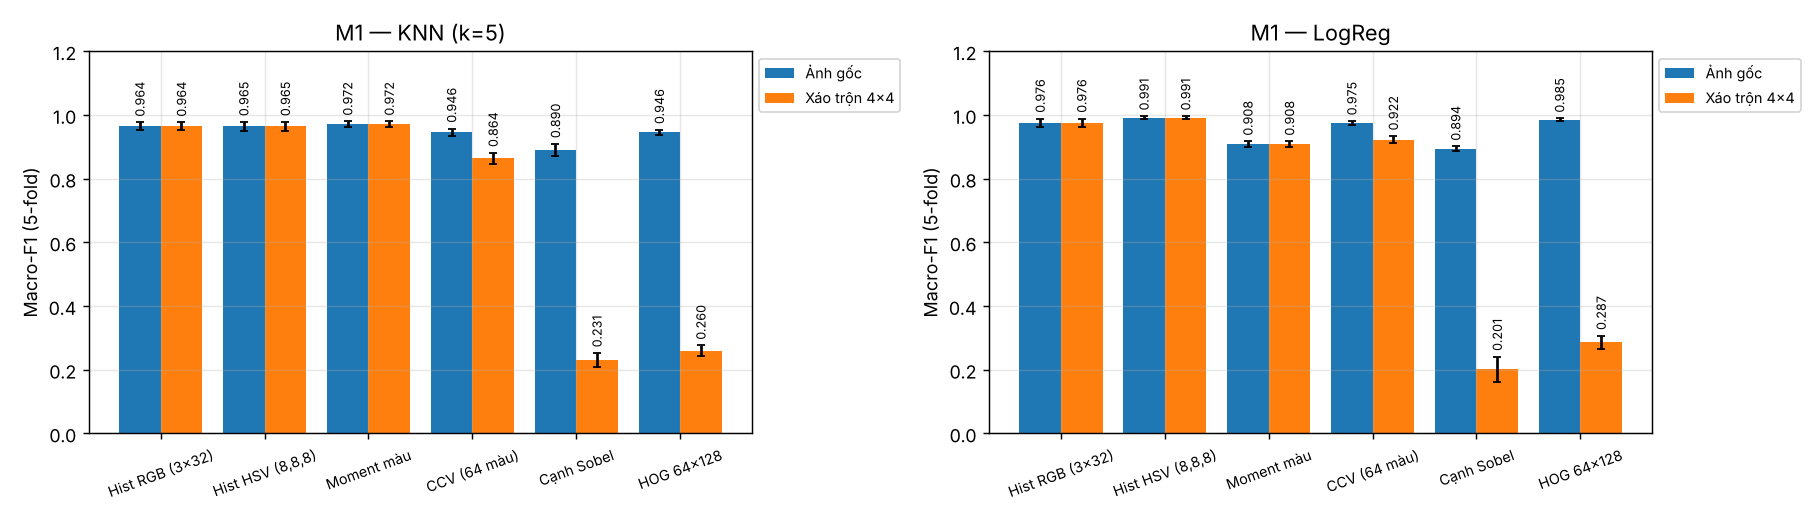
\includegraphics[width=\linewidth,height=0.72\textheight,keepaspectratio]{../results/figures/M1_shuffle.png}\end{center}
\end{column}
\end{columns}
\note{M1 khớp hoàn toàn: histogram không chứa thông tin vị trí. M2 khớp một phần: HSV đủ 3 kênh vẫn chứa V nên vẫn sụt mạnh; chỉ H-S bền. Bảng: results/M1/table.md, results/M2/table.md.}
\end{frame}

\begin{frame}{Phụ lục. M3-M6: Số bin, moment, CCV, ảnh xám}
\begin{columns}[T]
\begin{column}{0.36\textwidth}
\begin{itemize}\footnotesize
\item M3: 4 bin kém rõ; 16$^3$ bin làm KNN giảm (87\% phần tử = 0)
\item M4: moment 9 chiều: KNN 0.972 nhưng LogReg 0.908
\item M5: CCV nhạy bố cục nhưng không tốt hơn histogram
\item M6: học lại trên ảnh xám $\rightarrow$ màu sụt 0.04 đến 0.23; HOG vẫn 0.986
\end{itemize}
\end{column}
\begin{column}{0.62\textwidth}
\begin{center}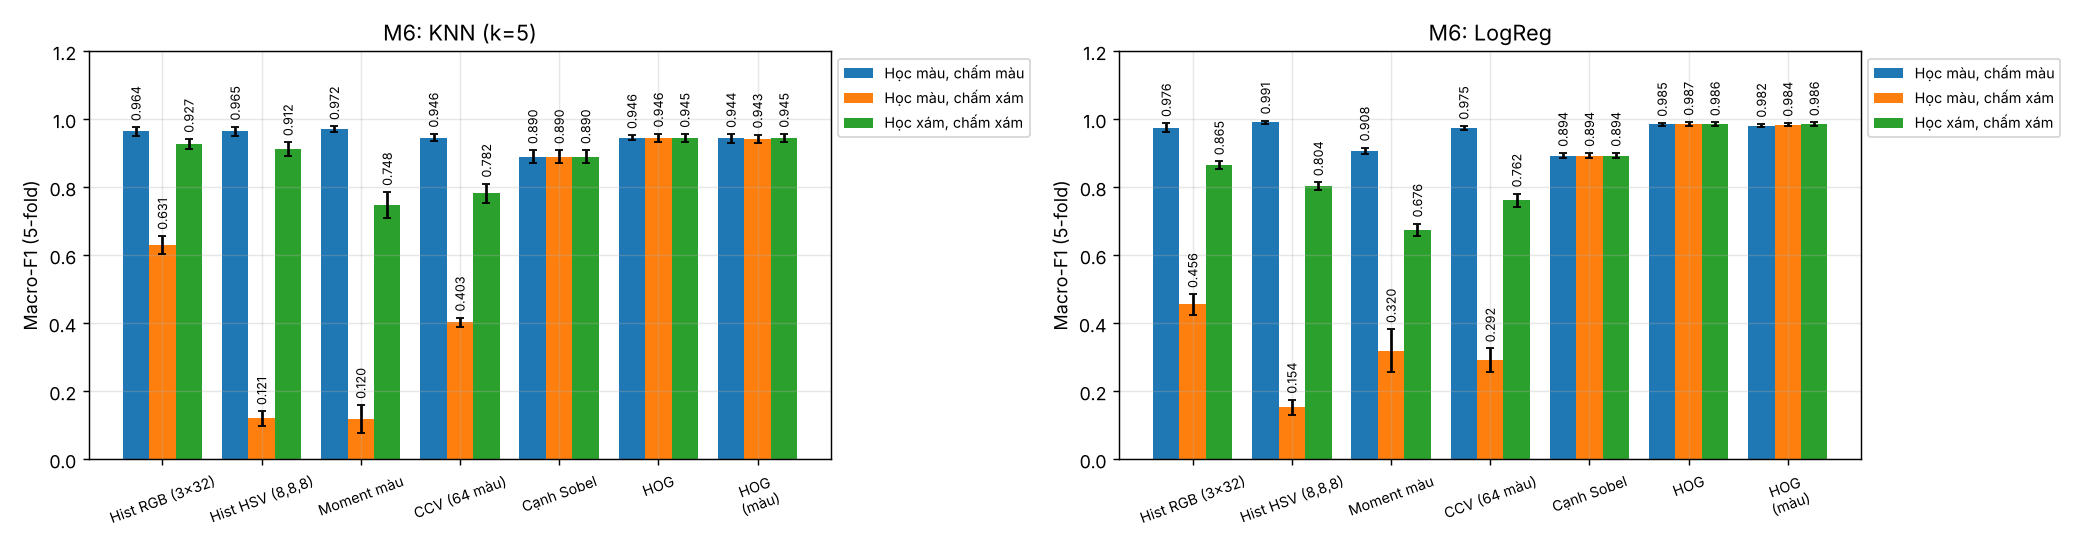
\includegraphics[width=\linewidth,height=0.72\textheight,keepaspectratio]{../results/figures/M6_grayscale.png}\end{center}
\end{column}
\end{columns}
\note{Hình là M6. Giống chuối phân biệt được cả bằng màu lẫn hình dạng. Moment màu ít chiều nên biên quyết định tuyến tính không đủ (liên hệ P6). CCV không giúp vì ảnh một quả nền trơn, hầu như mọi điểm ảnh đều thuộc vùng liên thông lớn.}
\end{frame}

\begin{frame}{Phụ lục. C1, C2: Toán tử cạnh và HOG}
\begin{columns}[T]
\begin{column}{0.36\textwidth}
\begin{itemize}\footnotesize
\item C1: $\sigma$ = 5 $\rightarrow$ vector đổi 43 đến 46\% (Prewitt/Sobel), 100\% (Roberts), 216\% (Laplacian): đúng thứ tự dự đoán
\item C2: chuẩn hóa block bền khi làm tối (sụt $\le$ 0.009)
\item Làm sáng V$\times$1.4: \textbf{trái dự đoán}: 68.7\% điểm ảnh bão hòa, 14.1\% cell mất gradient
\end{itemize}
\end{column}
\begin{column}{0.62\textwidth}
\begin{center}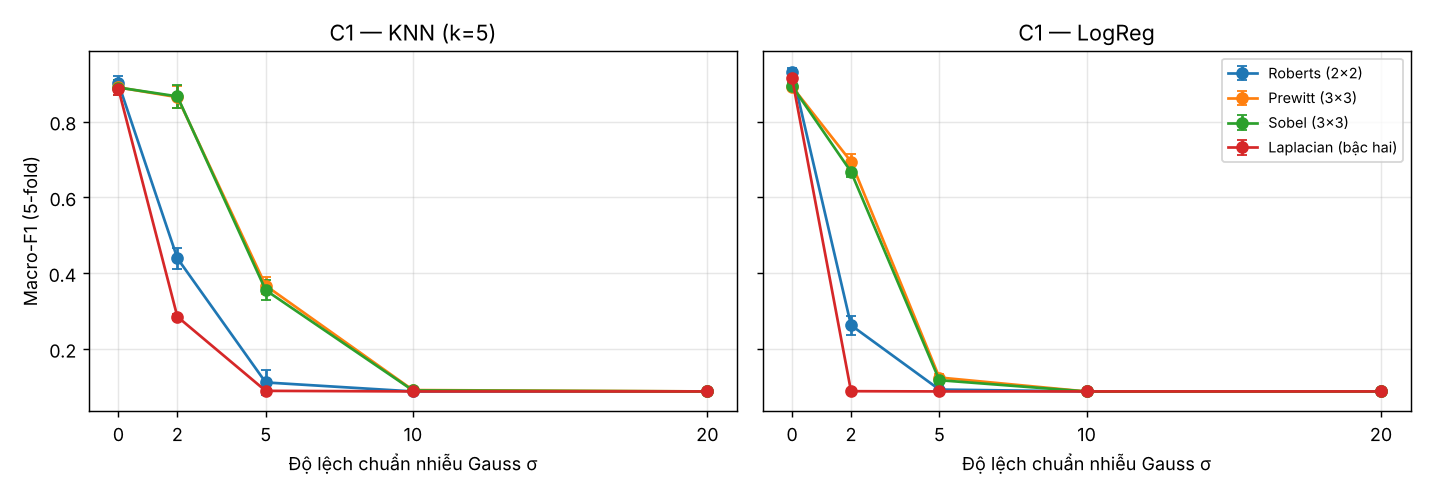
\includegraphics[width=\linewidth,height=0.72\textheight,keepaspectratio]{../results/figures/C1_edge_noise.png}\end{center}
\end{column}
\end{columns}
\note{C1 khớp lý thuyết: toán tử có làm trơn bền hơn, đạo hàm bậc hai nhạy nhất. C2: phép làm sáng gây bão hòa, không còn là phép nhân tuyến tính nên chuẩn hóa không khử được. Bảng: results/C1, results/C2.}
\end{frame}

\begin{frame}{Phụ lục. C3-C5: Tham số HOG, che 25\%, ghép đặc trưng}
\begin{columns}[T]
\begin{column}{0.36\textwidth}
\begin{itemize}\footnotesize
\item C3: chỉ cell/kích thước ảnh tạo khác biệt; số bin không
\item C4: histogram sập khi che: do \textbf{z-score}; Hellinger chỉ sụt 0.012
\item C5: H-S + HOG: 0.996 $\pm$ 0.003 (màu riêng 0.991, HOG riêng 0.986)
\end{itemize}
\end{column}
\begin{column}{0.62\textwidth}
\begin{center}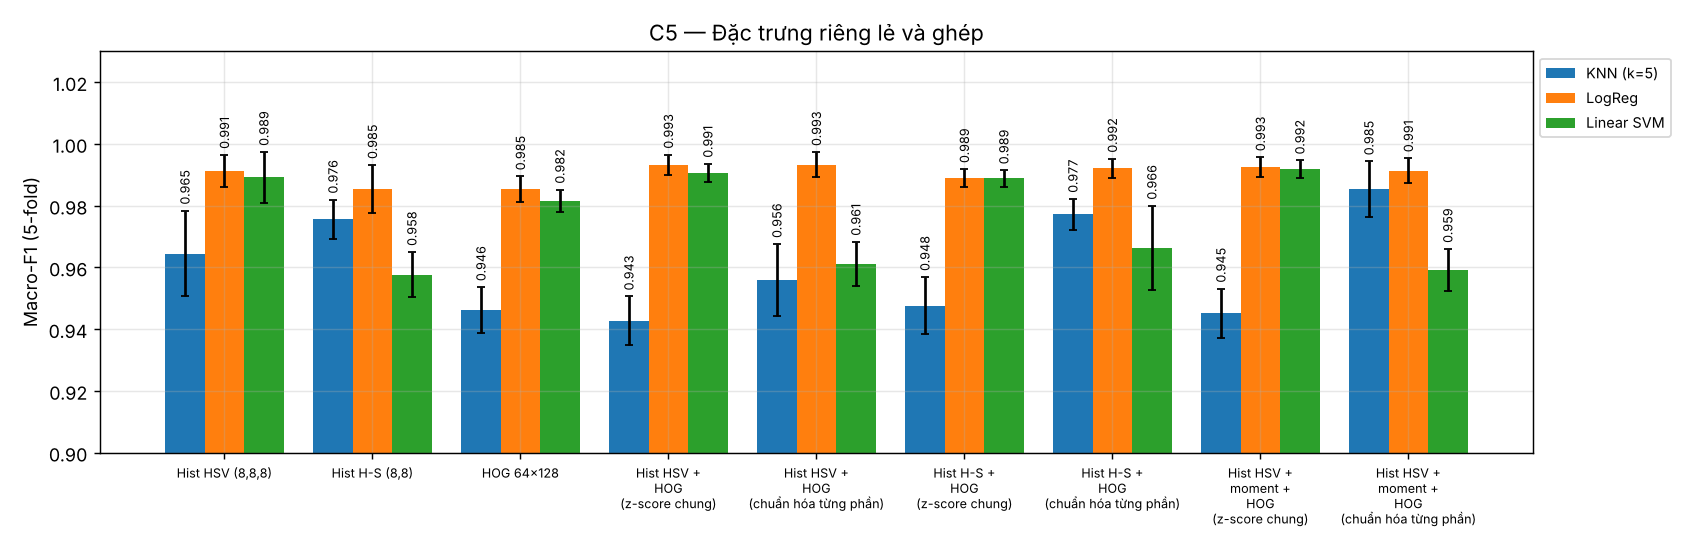
\includegraphics[width=\linewidth,height=0.72\textheight,keepaspectratio]{../results/figures/C5_fusion.png}\end{center}
\end{column}
\end{columns}
\note{C4 là ví dụ cho thấy kết luận phụ thuộc cả bước chuẩn hóa chứ không chỉ đặc trưng. C5: ghép màu và hình dạng tốt nhất, nhưng hơn màu riêng chỉ 0.005, bằng độ lệch chuẩn.}
\end{frame}

\begin{frame}{Phụ lục. P1-P3: KNN: k, độ đo, cách bình chọn}
\begin{columns}[T]
\begin{column}{0.36\textwidth}
\begin{itemize}\footnotesize
\item P1: k = 1 tốt nhất, hơn quy tắc k = 5 từ 0.006 đến 0.020
\item P2: chuẩn hóa đơn vị $\rightarrow$ Euclidean và cosine cùng 10 láng giềng ở 100\% ảnh
\item P3: uniform/distance chênh $\le$ 0.006 $\rightarrow$ chưa đủ cơ sở phân biệt
\end{itemize}
\end{column}
\begin{column}{0.62\textwidth}
\begin{center}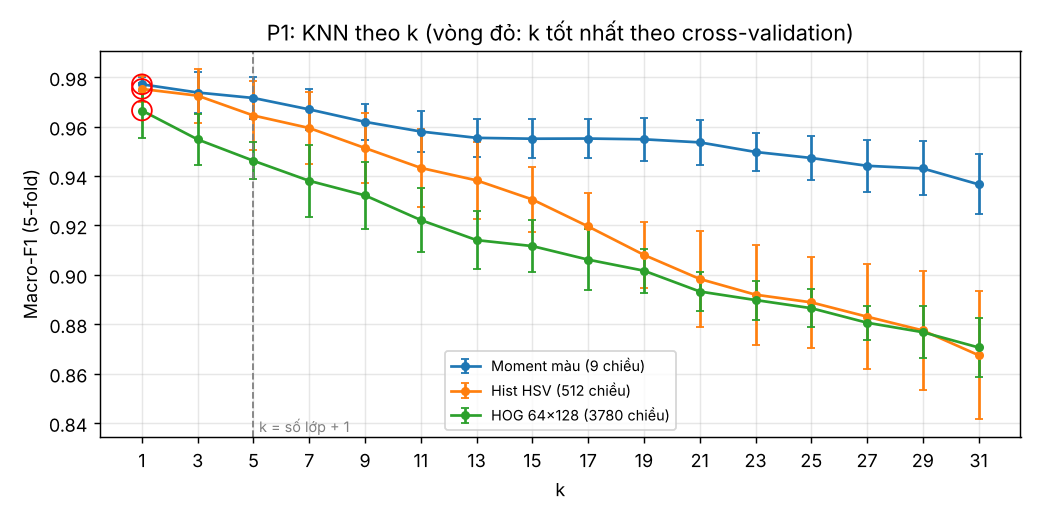
\includegraphics[width=\linewidth,height=0.72\textheight,keepaspectratio]{../results/figures/P1_knn_k.png}\end{center}
\end{column}
\end{columns}
\note{P1 trái với vế 'k nhỏ nhạy nhiễu' vì các lớp tách nhau rõ và có nhiều ảnh gần giống nhau. P2 kiểm chứng đúng điều lý thuyết dự đoán: trên vector đơn vị, khoảng cách Euclidean là hàm đơn điệu của cosine.}
\end{frame}

\begin{frame}{Phụ lục. P4-P6: Tốc độ và biên quyết định}
\begin{columns}[T]
\begin{column}{0.36\textwidth}
\begin{itemize}\footnotesize
\item P4: K-D Tree chậm hơn brute \textasciitilde{}60 lần ở 3780 chiều; chỉ nhanh hơn khi ít chiều và $\ge$ 8400 điểm
\item P5: KNN huấn luyện 0.07 s nhưng dự đoán 0.22 ms/ảnh; LogReg ngược lại
\item P6: 9 chiều: LogReg kém KNN 0.064; 3780 chiều: hơn 0.039
\end{itemize}
\end{column}
\begin{column}{0.62\textwidth}
\begin{center}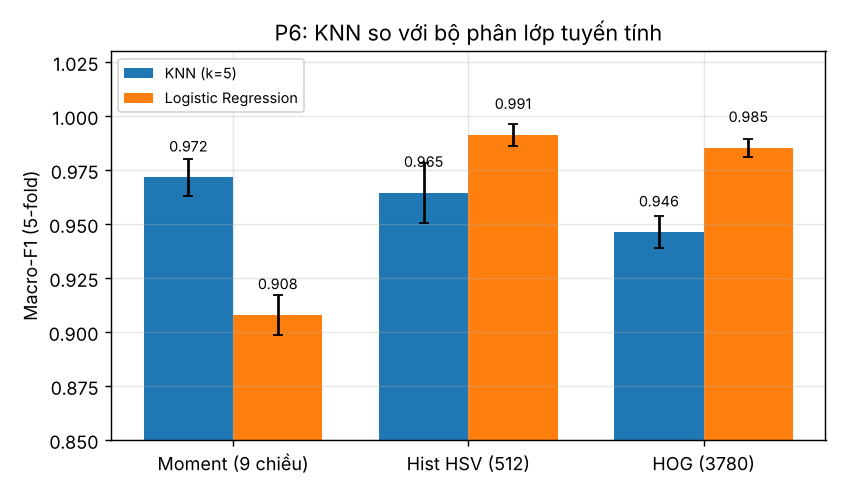
\includegraphics[width=\linewidth,height=0.72\textheight,keepaspectratio]{../results/figures/P6_linear_vs_knn.png}\end{center}
\end{column}
\end{columns}
\note{Kết quả của cây tìm kiếm luôn trùng brute force, chỉ khác tốc độ. Bộ phân lớp tuyến tính cần nhiều chiều để các lớp tách được.}
\end{frame}

\begin{frame}{Phụ lục. Cấu hình truyền thống đã chốt (5-fold CV)}
\begin{center}\begin{adjustbox}{max width=\linewidth,max totalheight=0.74\textheight}
\rowcolors{2}{uitbg}{white}
\begin{tabular}{llll}\toprule
\textbf{Vai trò} & \textbf{Cấu hình} & \textbf{Macro-F1 (5-fold)} & \textbf{Accuracy} \\ \midrule
trad\_color & Hist HSV (8,8,8) + LogReg C=0.1 & 0.991 $\pm$ 0.005 & 0.992 \\
trad\_edge & Cạnh Roberts + KNN k=1, Manhattan, ưu tiên điểm gần & 0.955 $\pm$ 0.015 & 0.959 \\
trad\_hog & HOG 64$\times$128 + LogReg C=0.1 & 0.986 $\pm$ 0.007 & 0.989 \\
trad\_fusion & Hist H-S + HOG + LogReg C=100, chuẩn hóa từng phần & 0.996 $\pm$ 0.003 & 0.997 \\
\bottomrule\end{tabular}
\end{adjustbox}\end{center}
\note{Sau khi quét siêu tham số: cấu hình ghép H-S + HOG + Logistic Regression tốt nhất, macro-F1 0.996 $\pm$ 0.003.}
\end{frame}

\begin{frame}{Phụ lục. Hướng A: N1, N2: tham số và lượng dữ liệu}
\begin{columns}[T]
\begin{column}{0.36\textwidth}
\begin{itemize}\footnotesize
\item N1: tính tay khớp 10/10 lớp; ví dụ conv2 của a\_lenet: (5$\times$5$\times$6+1)$\times$16 = 2416
\item Lớp Dense sau Flatten chiếm 96 đến 99\% số tham số
\item N2: 25\% $\rightarrow$ 100\% dữ liệu: a\_lenet +0.050; pretrained +0.016 đến 0.018
\end{itemize}
\end{column}
\begin{column}{0.62\textwidth}
\begin{center}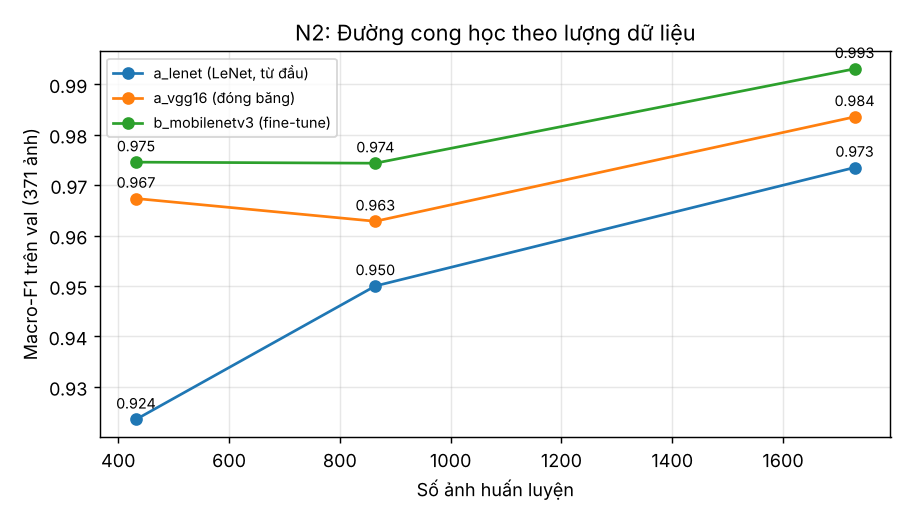
\includegraphics[width=\linewidth,height=0.72\textheight,keepaspectratio]{../results/figures/N2_learning_curve.png}\end{center}
\end{column}
\end{columns}
\note{Ví dụ tính tay số tham số. Đường cong học cho thấy mô hình học từ đầu cần nhiều dữ liệu hơn; với 25\% dữ liệu, mô hình pretrained đã ngang a\_lenet dùng đủ dữ liệu.}
\end{frame}

\begin{frame}{Phụ lục. Hướng A: N3, N5: Dropout và tăng cường ảnh}
\begin{columns}[T]
\begin{column}{0.36\textwidth}
\begin{itemize}\footnotesize
\item N3 (3 seed): có Dropout 0.941 $\pm$ 0.005; không Dropout 0.953 $\pm$ 0.006 $\rightarrow$ \textbf{trái dự đoán}
\item N5: tăng cường ảnh: khoảng cách loss val - train 0.542 $\rightarrow$ 0.054
\item Quá khớp nằm ở lớp Dense trước Dropout
\end{itemize}
\end{column}
\begin{column}{0.62\textwidth}
\begin{center}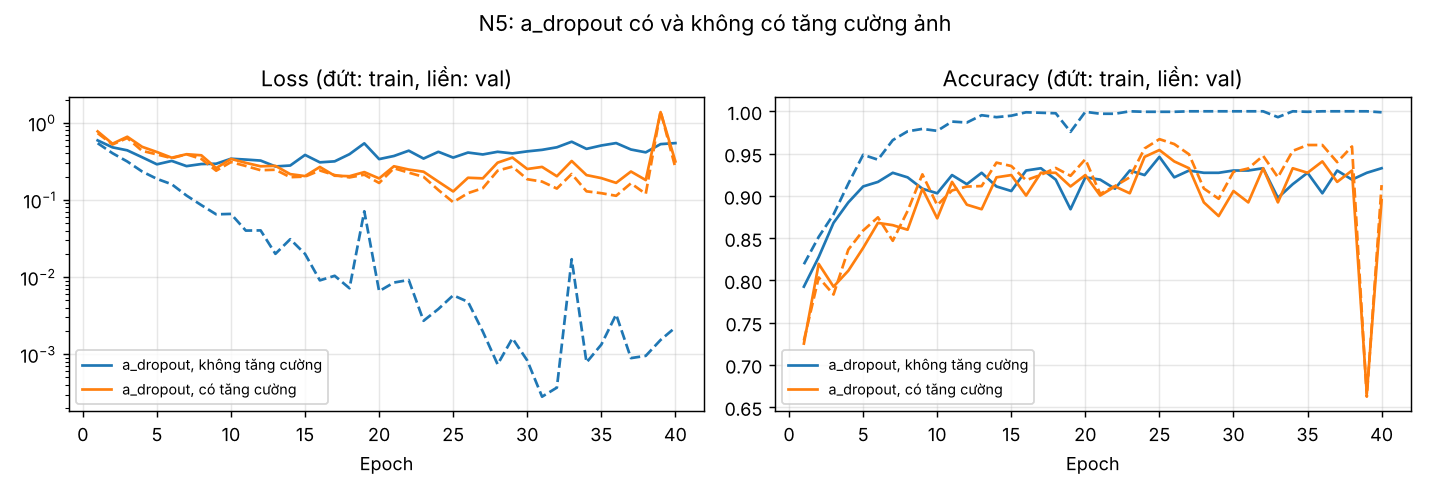
\includegraphics[width=\linewidth,height=0.72\textheight,keepaspectratio]{../results/figures/N5_augment_a_dropout.png}\end{center}
\end{column}
\end{columns}
\note{Dropout(0.5) đặt sau lớp Dense chứa 99\% tham số nên không chặn được quá khớp ở đó. Tăng cường ảnh tác động vào đầu vào nên hiệu quả hơn nhiều.}
\end{frame}

\begin{frame}{Phụ lục. Hướng B: N4: đóng băng và fine-tune}
\begin{columns}[T]
\begin{column}{0.36\textwidth}
\begin{itemize}\footnotesize
\item MobileNetV3: GĐ1 0.987 $\rightarrow$ GĐ2 0.993 (1e-5) / 1.000 (1e-4)
\item lr 1e-3: dao động, tụt tới 0.917
\item BatchNorm để mở khi fine-tune: embedding đổi 82\%, đầu phân lớp chỉ đúng 4.7\% $\rightarrow$ phải đóng băng BN
\end{itemize}
\end{column}
\begin{column}{0.62\textwidth}
\begin{center}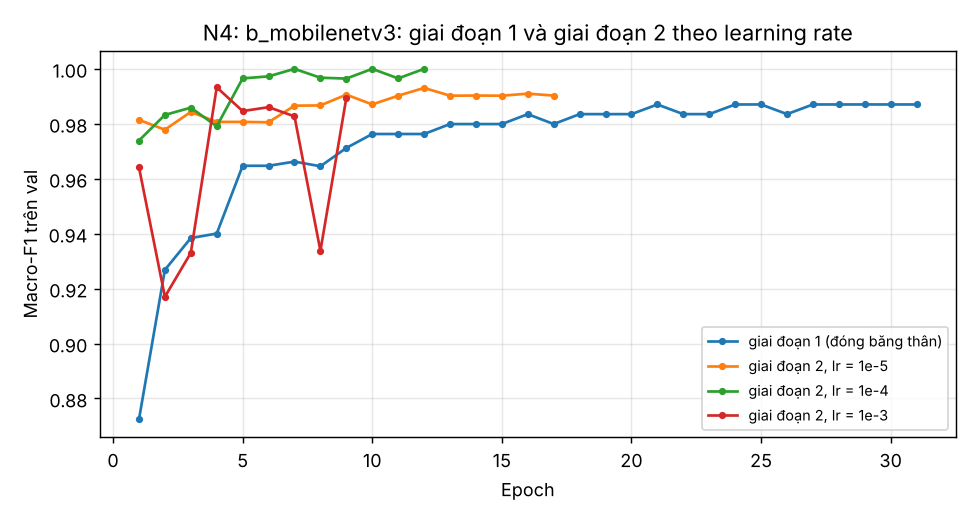
\includegraphics[width=\linewidth,height=0.72\textheight,keepaspectratio]{../results/figures/N4_finetune_lr.png}\end{center}
\end{column}
\end{columns}
\note{Fine-tune giúp nhưng mức tăng nhỏ vì giai đoạn 1 đã cao. Learning rate lớn làm mất ổn định. Chi tiết BatchNorm là bài học cài đặt quan trọng: results/N4/table\_batchnorm.md.}
\end{frame}

\begin{frame}{Phụ lục. N6: So sánh hướng A và hướng B}
\begin{center}\begin{adjustbox}{max width=\linewidth,max totalheight=0.74\textheight}
\rowcolors{2}{uitbg}{white}
\begin{tabular}{lllllll}\toprule
\textbf{Hướng} & \textbf{Mô hình} & \textbf{Macro-F1 val} & \textbf{Số tham số} & \textbf{File mô hình (MB)} & \textbf{Thời gian huấn luyện (s)} & \textbf{Dự đoán 1 ảnh (ms, CPU)} \\ \midrule
A & a\_lenet & 0.973 & 337976 & 1.4 & 30 & 1.4 \\
A & a\_dropout & 0.948 & 1746260 & 7.0 & 192 & 2.5 \\
A & a\_vgg16 & 0.990 & 40669252 & 162.8 & 226 & 130.4 \\
B & b\_mobilenetv3 & 1.000 & 941428 & 4.3 & 216 & 12.5 \\
B & b\_resnet50 & 0.998 & 23595908 & 95.1 & 591 & 61.1 \\
\bottomrule\end{tabular}
\end{adjustbox}\end{center}
\note{Hướng B tốt hơn. Nhưng 'lớn hơn' không có nghĩa là nặng hơn: MobileNetV3 chỉ 0.94 triệu tham số, 4.3 MB, 12.5 ms mỗi ảnh, trong khi a\_vgg16 của hướng A nặng 163 MB và mất 130 ms.}
\end{frame}

\begin{frame}{Phụ lục. N7, N8: Embedding và độ bền}
\begin{columns}[T]
\begin{column}{0.36\textwidth}
\begin{itemize}\footnotesize
\item N7: embedding MobileNetV3 đã fine-tune + KNN = 1.000; embedding ImageNet chưa học + KNN = 0.932
\item N8: CNN bền với nhiễu, xoay, ảnh xám
\item Che 25\%: MobileNetV3 0.659 $<$ HOG 0.801 (trái dự đoán)
\item Xáo trộn: a\_vgg16 (Flatten) 0.097; MobileNetV3 (GAP) 0.850
\end{itemize}
\end{column}
\begin{column}{0.62\textwidth}
\begin{center}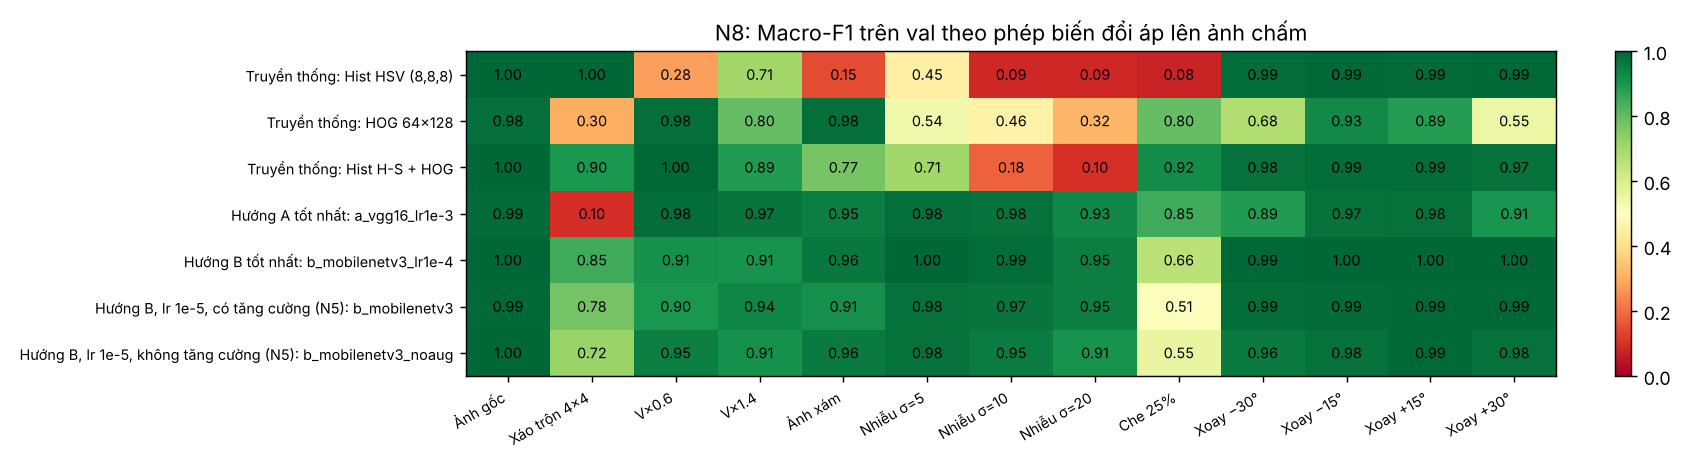
\includegraphics[width=\linewidth,height=0.72\textheight,keepaspectratio]{../results/figures/N8_robustness.png}\end{center}
\end{column}
\end{columns}
\note{Không phương pháp nào bền với mọi thay đổi; mỗi phương pháp bền với đúng loại thay đổi mà cấu trúc của nó bất biến.}
\end{frame}

\begin{frame}{Phụ lục. I1, I2: Mất cân bằng dữ liệu}
\begin{columns}[T]
\begin{column}{0.36\textwidth}
\begin{itemize}\footnotesize
\item I1: luôn đoán lớp đông nhất: accuracy 0.402, macro-F1 0.143
\item KNN k=31: accuracy 0.884 nhưng recall Sagor 0.552
\item I2: ở mô hình yếu, các cách xử lý đổi precision lấy recall; ở mô hình mạnh không tác động
\end{itemize}
\end{column}
\begin{column}{0.62\textwidth}
\begin{center}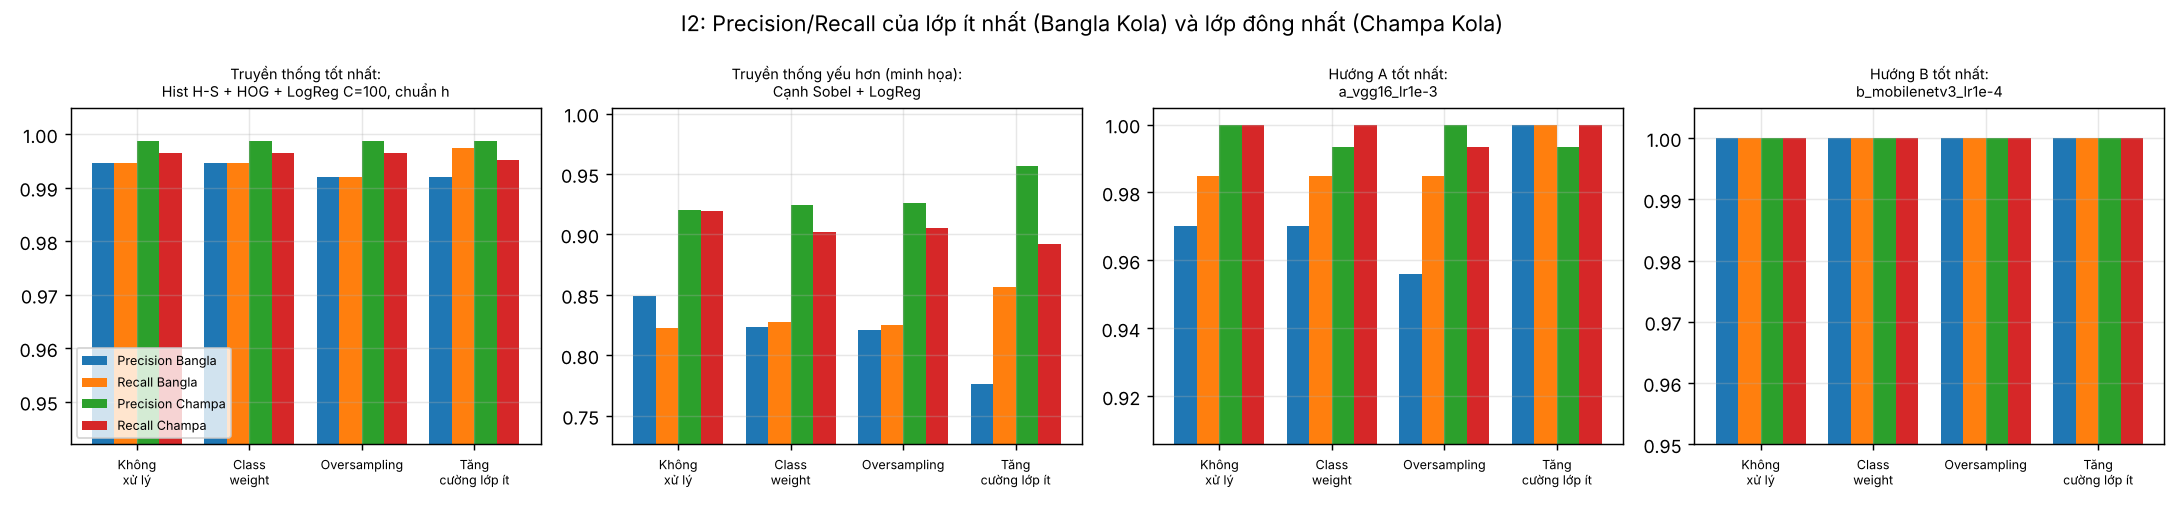
\includegraphics[width=\linewidth,height=0.72\textheight,keepaspectratio]{../results/figures/I2_imbalance.png}\end{center}
\end{column}
\end{columns}
\note{Accuracy có thể che khuất lớp bị nhận kém; vì vậy chỉ số chính là macro-F1. Với tỉ lệ 2.2 lần, mất cân bằng không phải vấn đề chính.}
\end{frame}

\begin{frame}{Phụ lục. S1: Phân đoạn tách nền}
\begin{center}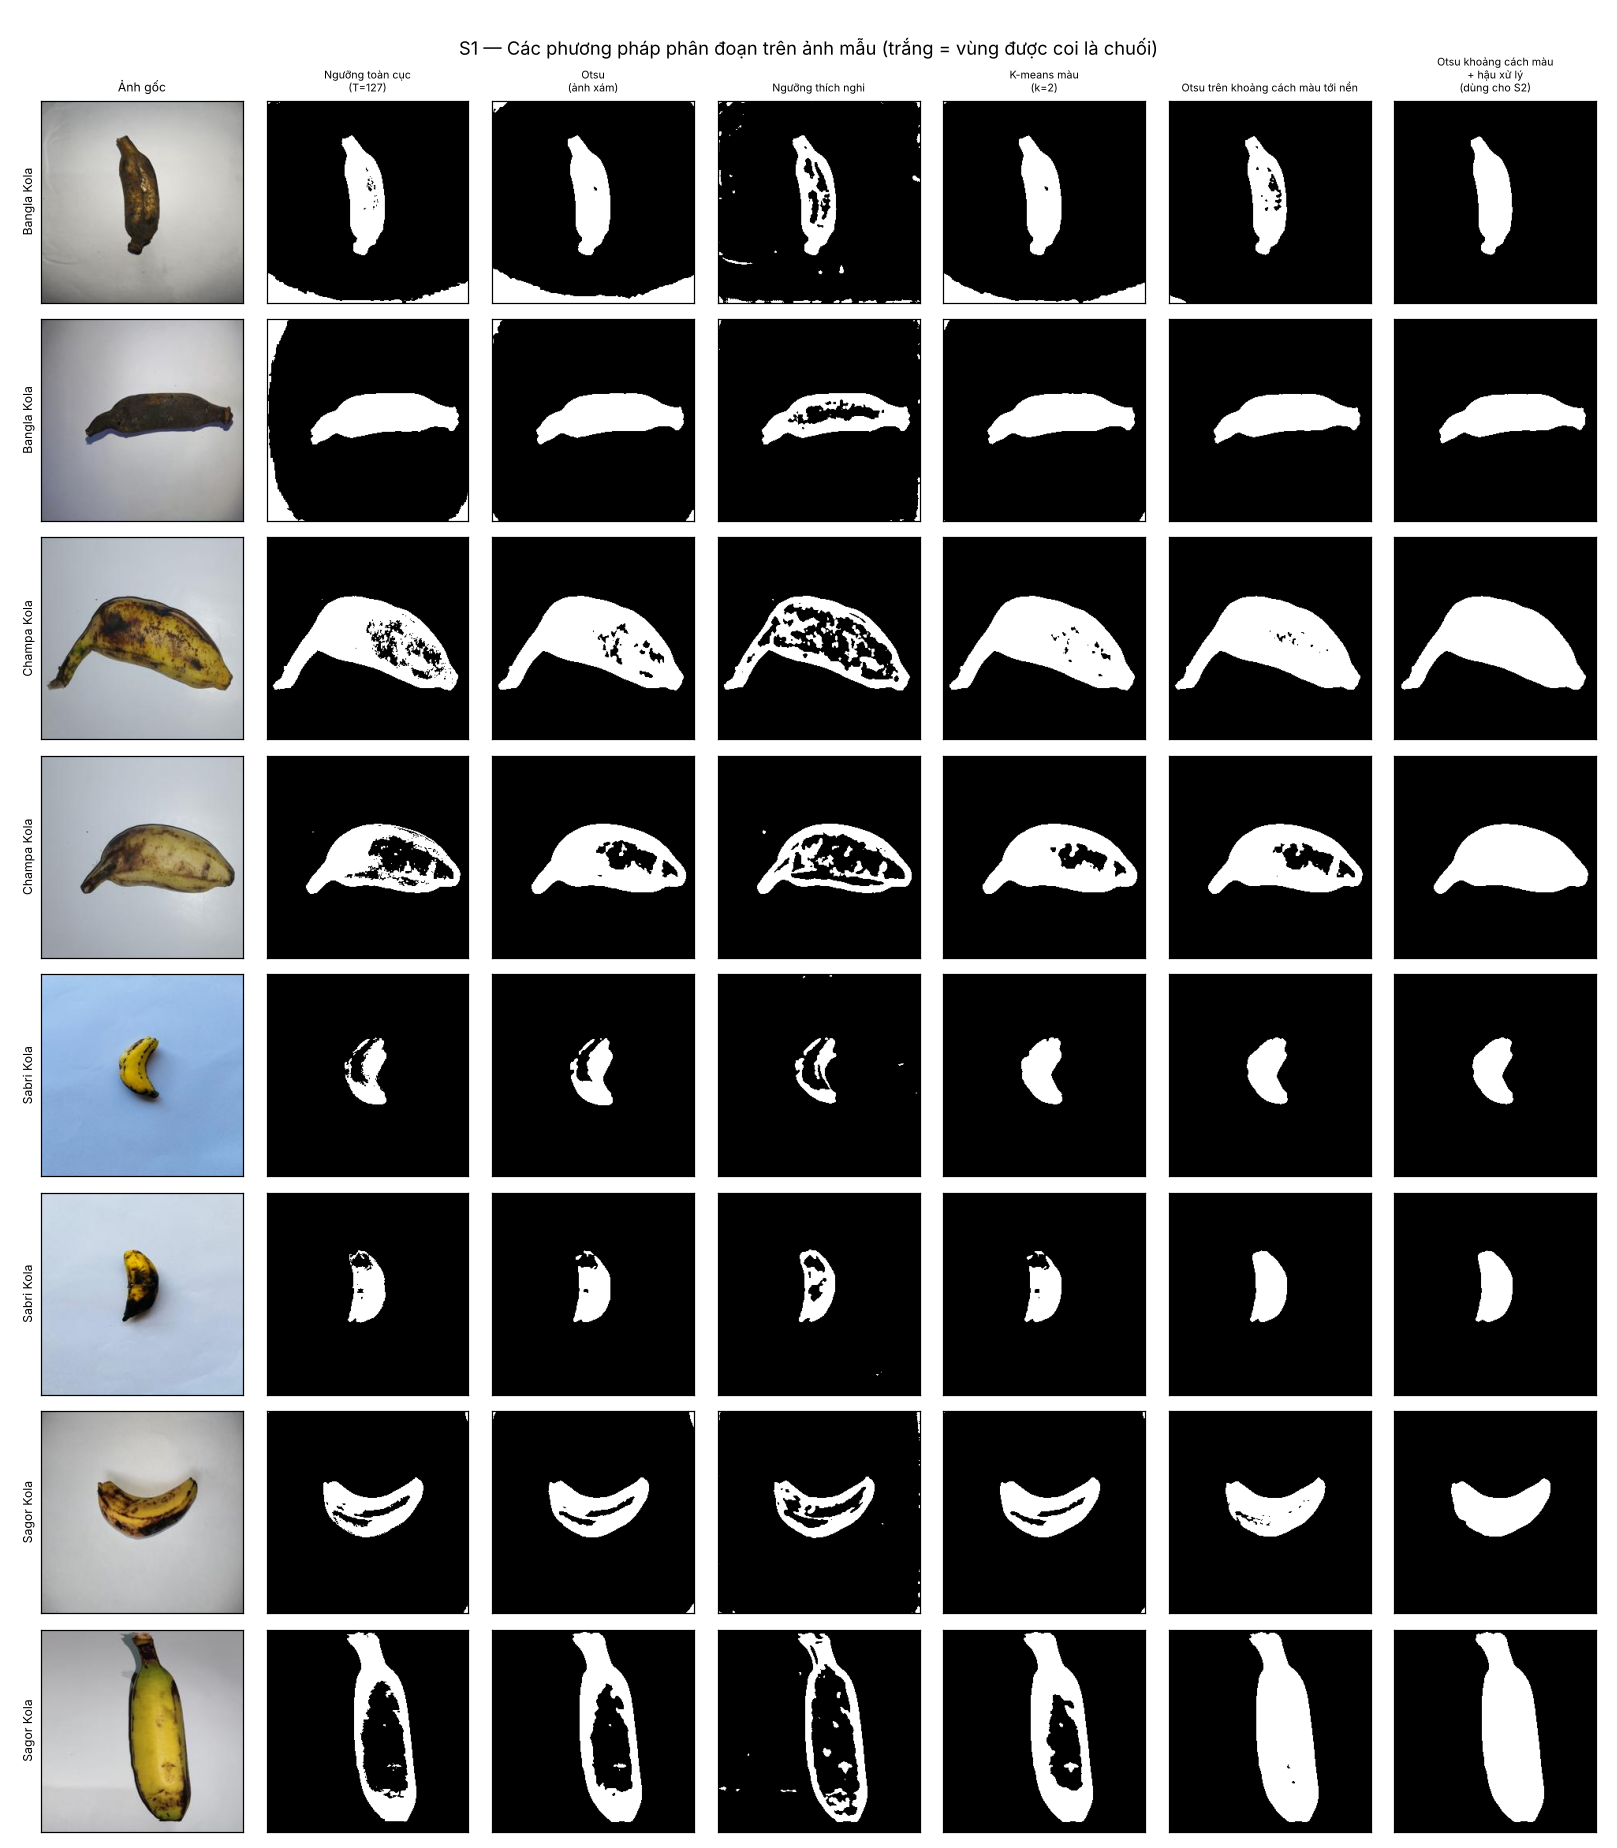
\includegraphics[width=\linewidth,height=0.74\textheight,keepaspectratio]{../results/figures/S1_segmentation.png}\end{center}
\note{Ngưỡng toàn cục và thích nghi tách cả vết thâm thành nền. Các cách dựa trên màu (k-means, Otsu trên khoảng cách màu tới nền) cho mask liền nhất. Không có nhãn mask nên đánh giá định tính, kèm số mảnh rời và tỉ lệ lỗ thủng.}
\end{frame}

\begin{frame}{Phụ lục. S2: Mô hình dựa vào quả chuối hay vào nền?}
\begin{columns}[T]
\begin{column}{0.36\textwidth}
\begin{itemize}\footnotesize
\item Chỉ 4 góc ảnh 64$\times$64: HOG 0.968; histogram 0.939
\item Chỉ 3 số màu nền + KNN: 0.937
\item CNN đoán trên ảnh đã xóa quả: 0.683 đến 0.792
\item \textbf{Dữ liệu thiên lệch theo bối cảnh chụp}
\item Chỉ nhìn quả: truyền thống 0.958, CNN 0.926 đến 0.952
\end{itemize}
\end{column}
\begin{column}{0.62\textwidth}
\begin{center}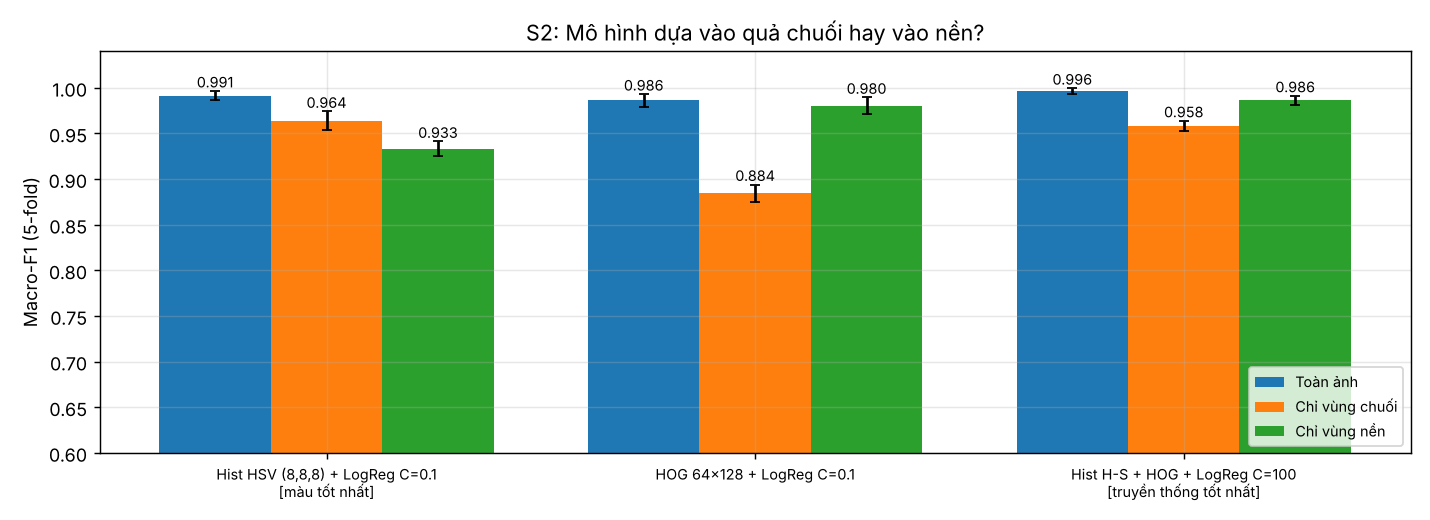
\includegraphics[width=\linewidth,height=0.72\textheight,keepaspectratio]{../results/figures/S2_background_bias.png}\end{center}
\end{column}
\end{columns}
\note{Đây là phát hiện quan trọng nhất. Mỗi giống được chụp trong điều kiện riêng: nền Sabri xanh hơn, quả Sabri chiếm 5.4\% ảnh so với 22\% ở Sagor. Vì vậy con số gần 100\% là độ chính xác trên bộ dữ liệu này, không phải trong điều kiện bất kỳ.}
\end{frame}

\begin{frame}{Phụ lục. Kết quả cuối trên tập test (371 ảnh)}
\begin{center}\begin{adjustbox}{max width=\linewidth,max totalheight=0.74\textheight}
\rowcolors{2}{uitbg}{white}
\begin{tabular}{llllll}\toprule
\textbf{Nhóm} & \textbf{Mô hình} & \textbf{Macro-F1 test} & \textbf{KTC 95\% (bootstrap)} & \textbf{Accuracy test} & \textbf{Số ảnh sai / 371} \\ \midrule
Truyền thống (màu) & Hist HSV (8,8,8) + LogReg C=0.1 & 0.994 & [0.984; 1.000] & 0.995 & 2 \\
Truyền thống (cạnh) & Cạnh Roberts + KNN k=1, Manhattan, ưu tiên điểm gần & 0.964 & [0.944; 0.982] & 0.968 & 12 \\
Truyền thống (HOG) & HOG 64$\times$128 + LogReg C=0.1 & 0.990 & [0.977; 1.000] & 0.992 & 3 \\
Truyền thống (ghép) & Hist H-S + HOG + LogReg C=100, chuẩn hóa từng phần & 1.000 & [1.000; 1.000] & 1.000 & 0 \\
CNN hướng A & a\_lenet (biến thể: a\_lenet) & 0.978 & [0.960; 0.993] & 0.981 & 7 \\
CNN hướng A & a\_dropout (biến thể: a\_dropout\_aug) & 0.942 & [0.917; 0.965] & 0.943 & 21 \\
CNN hướng A & a\_vgg16 (biến thể: a\_vgg16\_lr1e-3) & 0.986 & [0.971; 0.997] & 0.989 & 4 \\
CNN hướng B & b\_mobilenetv3 (biến thể: b\_mobilenetv3\_lr1e-4) & 1.000 & [1.000; 1.000] & 1.000 & 0 \\
CNN hướng B & b\_resnet50 (biến thể: b\_resnet50) & 0.997 & [0.988; 1.000] & 0.997 & 1 \\
\bottomrule\end{tabular}
\end{adjustbox}\end{center}
\note{Truyền thống tốt nhất (H-S + HOG + LogReg) và b\_mobilenetv3 đều đúng 371/371 ảnh, macro-F1 1.000 và 1.000. a\_vgg16 tốt nhất hướng A với 0.986. Khoảng tin cậy chồng lên nhau nên không tuyên bố hơn kém giữa các mô hình dẫn đầu.}
\end{frame}

\begin{frame}{Phụ lục. Phân tích lỗi}
\begin{columns}[T]
\begin{column}{0.36\textwidth}
\begin{itemize}\footnotesize
\item 41 ảnh test bị ít nhất 1/9 mô hình đoán sai
\item Nhầm nhiều nhất: Sagor $\rightarrow$ Champa
\item Ảnh Sagor bị sai có quả nhỏ hơn trung bình lớp (0.181 so với 0.244)
\item Sabri\_Kola\_5: quả to, nền trắng $\rightarrow$ 6/9 mô hình sai
\end{itemize}
\end{column}
\begin{column}{0.62\textwidth}
\begin{center}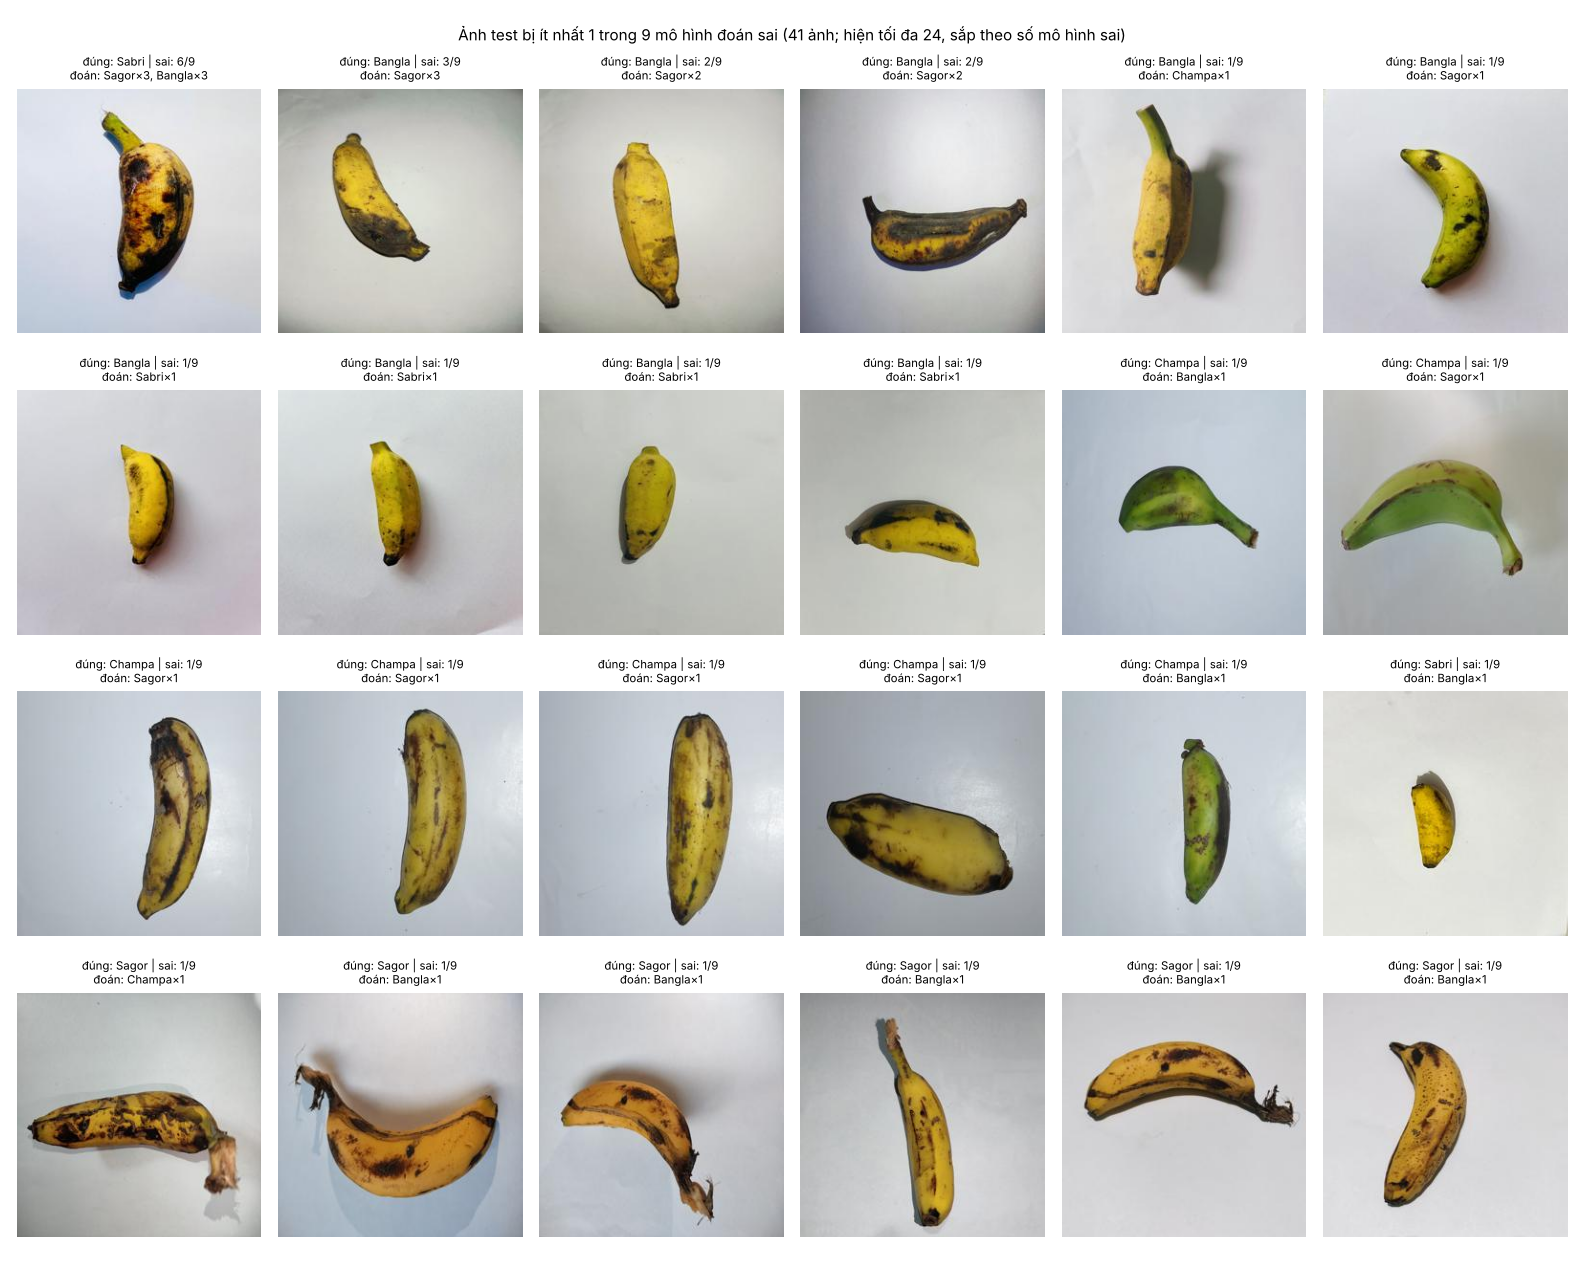
\includegraphics[width=\linewidth,height=0.72\textheight,keepaspectratio]{../results/figures/final_errors_all.png}\end{center}
\end{column}
\end{columns}
\note{Lỗi khớp với thiên lệch đo ở S2: ảnh không giống ảnh điển hình của lớp về kích thước quả và nền thì dễ bị đoán sai.}
\end{frame}

\begin{frame}{Phụ lục. Mở rộng: ba nhánh độc lập và bộ kiểm tra khó}
\begin{columns}[T]
\begin{column}{0.36\textwidth}
\begin{itemize}\footnotesize
\item \textbf{G}: pipeline gốc (mốc)
\item \textbf{X}: xử lý dữ liệu do nhóm thiết kế
\item \textbf{T}: bản Augmented của tác giả bộ dữ liệu
\item \textbf{B}: phương pháp của bài báo (Ergün 2025)
\item Mỗi nhánh đổi một thứ so với G; cùng 371 ảnh test gốc
\item Bộ kiểm tra khó: 6 phép biến đổi; \textbf{điểm bền} = trung bình macro-F1
\end{itemize}
\end{column}
\begin{column}{0.62\textwidth}
\begin{center}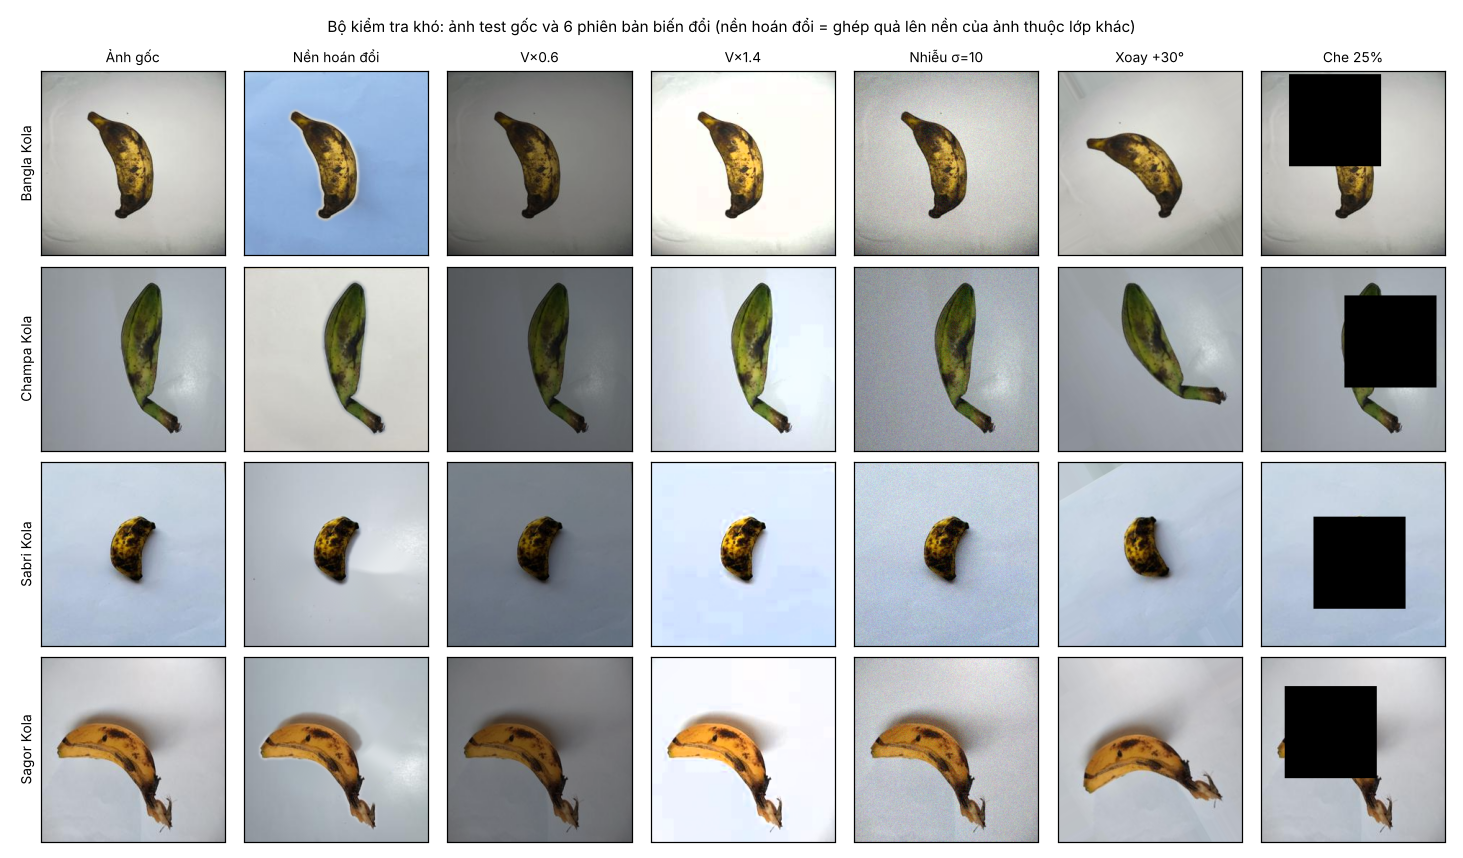
\includegraphics[width=\linewidth,height=0.72\textheight,keepaspectratio]{../results/figures/E_stress_examples.png}\end{center}
\end{column}
\end{columns}
\note{Trên ảnh gốc, hai cấu hình của pipeline gốc đã đúng 371/371 ảnh nên không còn chỗ để so sánh. Vì vậy mỗi mô hình được chấm thêm trên 6 phiên bản biến đổi của tập test, trong đó nền hoán đổi là ghép quả chuối lên nền của ảnh thuộc lớp khác. Ba nhánh độc lập, không chồng lên nhau.}
\end{frame}

\begin{frame}{Phụ lục. Nhánh G trên bộ kiểm tra khó}
\begin{center}\begin{adjustbox}{max width=\linewidth,max totalheight=0.74\textheight}
\rowcolors{2}{uitbg}{white}
\begin{tabular}{lllllllll}\toprule
\textbf{Mô hình} & \textbf{Macro-F1 test} & \textbf{Nền hoán đổi} & \textbf{V$\times$0.6} & \textbf{V$\times$1.4} & \textbf{Nhiễu $\sigma$=10} & \textbf{Xoay +30$^\circ$} & \textbf{Che 25\%} & \textbf{Điểm bền} \\ \midrule
Hist HSV (8,8,8) + LogReg C=0.1 & 0.994 & 0.726 & 0.304 & 0.673 & 0.086 & 0.983 & 0.150 & 0.487 \\
Cạnh Roberts + KNN k=1, Manhattan, ưu tiên điểm gần & 0.964 & 0.759 & 0.691 & 0.901 & 0.085 & 0.730 & 0.755 & 0.654 \\
HOG 64$\times$128 + LogReg C=0.1 & 0.990 & 0.145 & 0.987 & 0.776 & 0.484 & 0.505 & 0.805 & 0.617 \\
Hist H-S + HOG + LogReg C=100, chuẩn hóa từng phần & 1.000 & 0.410 & 0.997 & 0.856 & 0.172 & 0.972 & 0.959 & 0.728 \\
a\_lenet & 0.978 & 0.744 & 0.979 & 0.977 & 0.978 & 0.874 & 0.469 & 0.837 \\
a\_dropout & 0.942 & 0.855 & 0.864 & 0.932 & 0.940 & 0.925 & 0.100 & 0.769 \\
a\_vgg16 & 0.986 & 0.657 & 0.979 & 0.963 & 0.984 & 0.887 & 0.843 & 0.886 \\
b\_mobilenetv3 & 1.000 & 0.794 & 0.919 & 0.890 & 0.989 & 1.000 & 0.659 & 0.875 \\
b\_resnet50 & 0.997 & 0.792 & 0.916 & 0.966 & 0.990 & 0.993 & 0.714 & 0.895 \\
\bottomrule\end{tabular}
\end{adjustbox}\end{center}
\note{Macro-F1 trên ảnh gốc 0.94 đến 1.00 nhưng điểm bền chỉ 0.49 đến 0.90. Nền hoán đổi làm mọi cấu hình tụt: HOG còn 0.145, cấu hình truyền thống tốt nhất còn 0.410, b\_mobilenetv3 còn 0.794. Đây là xác nhận thứ hai cho kết luận của S2: mô hình dựa một phần vào nền.}
\end{frame}

\begin{frame}{Phụ lục. Nhánh X: làm sạch dữ liệu (X1)}
\begin{columns}[T]
\begin{column}{0.36\textwidth}
\begin{itemize}\footnotesize
\item Loại 35 ảnh train gần trùng (15 trùng với val/test, 20 lặp trong train)
\item Mask của S1 tràn nền ở 5.2\% ảnh $\rightarrow$ dùng mô hình nền bậc hai
\item Bài báo dữ liệu: \textbf{mỗi quả chụp 4 mặt}
\item 20\% ảnh có láng giềng gần nhất mang số thứ tự liền kề (ngẫu nhiên: 1\%)
\item Chia theo khối ảnh liên tiếp thấp hơn chia ngẫu nhiên 0.02 đến 0.07
\end{itemize}
\end{column}
\begin{column}{0.62\textwidth}
\begin{center}\begin{adjustbox}{max width=\linewidth,max totalheight=0.74\textheight}
\rowcolors{2}{uitbg}{white}
\begin{tabular}{llll}\toprule
\textbf{Mô hình} & \textbf{5-fold ngẫu nhiên phân tầng} & \textbf{5-fold theo khối ảnh liên tiếp} & \textbf{Chênh} \\ \midrule
Hist HSV (8,8,8) + LogReg C=0.1 & 0.991 $\pm$ 0.005 & 0.922 $\pm$ 0.042 & +0.069 \\
HOG 64$\times$128 + LogReg C=0.1 & 0.986 $\pm$ 0.007 & 0.933 $\pm$ 0.062 & +0.053 \\
Hist H-S + HOG + LogReg C=100 & 0.996 $\pm$ 0.003 & 0.973 $\pm$ 0.017 & +0.024 \\
Embedding MobileNetV3 (ImageNet) + LogReg & 0.995 $\pm$ 0.005 & 0.964 $\pm$ 0.025 & +0.031 \\
\bottomrule\end{tabular}
\end{adjustbox}\end{center}
\end{column}
\end{columns}
\note{Pipeline gốc chỉ resize ảnh. Bước làm sạch loại ảnh gần trùng khỏi train. Phát hiện quan trọng: ảnh cùng quả hoặc cùng đợt chụp nằm ở cả hai phía khi chia ngẫu nhiên, nên cross-validation ngẫu nhiên lạc quan hơn chia theo khối ảnh liên tiếp. Bảng: results/E1\_xu\_ly/table\_blocked\_cv.md, table\_adjacent.md.}
\end{frame}

\begin{frame}{Phụ lục. Nhánh X: chọn tiền xử lý và tăng cường trên val (X2-X4)}
\begin{columns}[T]
\begin{column}{0.36\textwidth}
\begin{itemize}\footnotesize
\item 5 mức tiền xử lý $\times$ 3 mức tăng cường, 7 phép thử trên val
\item Không xử lý: điểm chọn 0.804
\item \textbf{X-a} (cao nhất): nền phẳng (không cân bằng trắng) + hình học + quang học: 0.889 $\pm$ 0.006
\item \textbf{X-b} (chỉ can thiệp train): hình học + quang học + thay nền ngẫu nhiên: 0.835
\item Cân bằng trắng theo nền làm kém đi: đưa màu nền vào màu quả (X3)
\item Cắt theo quả làm phép che 25\% tệ hơn
\end{itemize}
\end{column}
\begin{column}{0.62\textwidth}
\begin{center}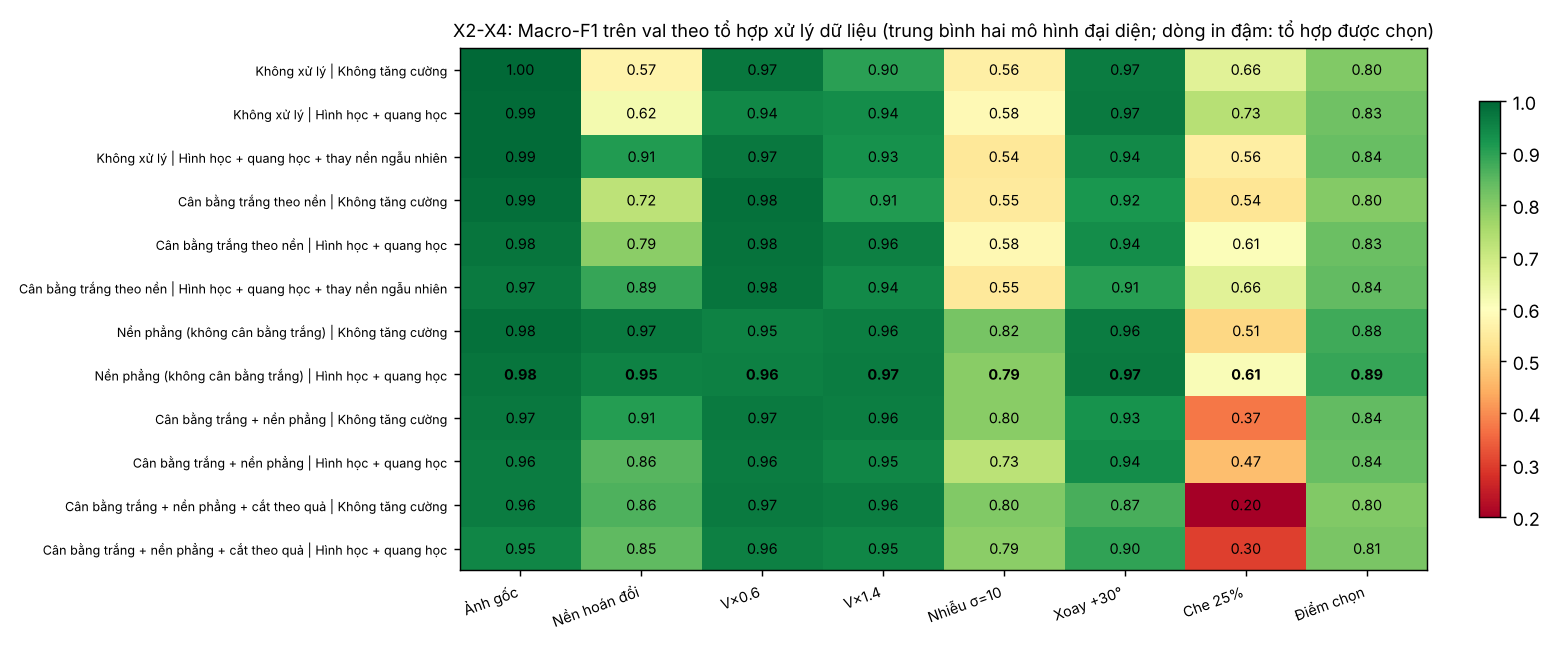
\includegraphics[width=\linewidth,height=0.72\textheight,keepaspectratio]{../results/figures/E1_selection.png}\end{center}
\end{column}
\end{columns}
\note{Điểm chọn là trung bình macro-F1 trên val của ảnh gốc và 6 phép thử khó, với hai mô hình đại diện; sai số tính bằng bootstrap. Tách nền (nền phẳng) là bước có tác dụng lớn nhất. Cân bằng trắng theo nền bị loại: hệ số tính từ màu nền rồi nhân vào cả quả chuối, nên khi nền đổi thì màu quả lệch 12.9 đơn vị Lab. Nhóm chạy đủ pipeline cho hai biến thể X-a và X-b. Bảng: results/E1\_xu\_ly/table\_selection.md, table\_wb\_leak.md.}
\end{frame}

\begin{frame}{Phụ lục. Nhánh X-a: 9 cấu hình với nền phẳng + tăng cường}
\begin{center}\begin{adjustbox}{max width=\linewidth,max totalheight=0.74\textheight}
\rowcolors{2}{uitbg}{white}
\begin{tabular}{lllllllll}\toprule
\textbf{Mô hình} & \textbf{Macro-F1 test} & \textbf{Nền hoán đổi} & \textbf{V$\times$0.6} & \textbf{V$\times$1.4} & \textbf{Nhiễu $\sigma$=10} & \textbf{Xoay +30$^\circ$} & \textbf{Che 25\%} & \textbf{Điểm bền} \\ \midrule
Hist HSV (8,8,8) + LogReg C=0.1 & 0.993 & 0.966 & 0.834 & 0.784 & 0.354 & 0.993 & 0.169 & 0.683 \\
Cạnh Roberts + KNN k=1, Manhattan, ưu tiên điểm gần & 0.842 & 0.838 & 0.799 & 0.820 & 0.792 & 0.686 & 0.381 & 0.719 \\
HOG 64$\times$128 + LogReg C=0.1 & 0.828 & 0.836 & 0.810 & 0.831 & 0.822 & 0.629 & 0.294 & 0.704 \\
Hist H-S + HOG + LogReg C=100, chuẩn hóa từng phần & 0.982 & 0.951 & 0.978 & 0.979 & 0.651 & 0.974 & 0.805 & 0.890 \\
a\_lenet & 0.922 & 0.925 & 0.861 & 0.846 & 0.922 & 0.797 & 0.317 & 0.778 \\
a\_dropout & 0.959 & 0.959 & 0.880 & 0.942 & 0.962 & 0.946 & 0.207 & 0.816 \\
a\_vgg16 & 0.958 & 0.951 & 0.933 & 0.954 & 0.964 & 0.926 & 0.413 & 0.857 \\
b\_mobilenetv3 & 0.995 & 0.995 & 0.943 & 0.915 & 0.988 & 0.998 & 0.450 & 0.881 \\
b\_resnet50 & 0.997 & 0.997 & 0.983 & 0.956 & 0.985 & 0.990 & 0.397 & 0.885 \\
\bottomrule\end{tabular}
\end{adjustbox}\end{center}
\note{X-a: thay nền bằng màu trắng phẳng, giữ nguyên màu quả, áp dụng cho cả ảnh train lẫn ảnh cần dự đoán; train được thêm 2 bản tăng cường mỗi ảnh. Cột nền hoán đổi gần bằng cột ảnh gốc ở mọi cấu hình: mô hình không còn dựa vào nền. Đổi lại HOG, cạnh, a\_lenet, a\_vgg16 mất điểm trên ảnh gốc, và phép che 25\% làm hỏng bước phân đoạn.}
\end{frame}

\begin{frame}{Phụ lục. Nhánh X-b: tăng cường có thay nền ngẫu nhiên (6 cấu hình)}
\begin{center}\begin{adjustbox}{max width=\linewidth,max totalheight=0.74\textheight}
\rowcolors{2}{uitbg}{white}
\begin{tabular}{lllllllll}\toprule
\textbf{Mô hình} & \textbf{Macro-F1 test} & \textbf{Nền hoán đổi} & \textbf{V$\times$0.6} & \textbf{V$\times$1.4} & \textbf{Nhiễu $\sigma$=10} & \textbf{Xoay +30$^\circ$} & \textbf{Che 25\%} & \textbf{Điểm bền} \\ \midrule
Hist HSV (8,8,8) + LogReg C=0.1 & 0.988 & 0.963 & 0.459 & 0.714 & 0.184 & 0.982 & 0.143 & 0.574 \\
Cạnh Roberts + KNN k=1, Manhattan, ưu tiên điểm gần & 0.960 & 0.799 & 0.691 & 0.892 & 0.179 & 0.708 & 0.617 & 0.648 \\
HOG 64$\times$128 + LogReg C=0.1 & 0.953 & 0.495 & 0.922 & 0.720 & 0.662 & 0.615 & 0.571 & 0.664 \\
Hist H-S + HOG + LogReg C=100, chuẩn hóa từng phần & 0.984 & 0.853 & 0.977 & 0.930 & 0.128 & 0.908 & 0.842 & 0.773 \\
a\_vgg16 & 0.977 & 0.907 & 0.960 & 0.953 & 0.965 & 0.943 & 0.516 & 0.874 \\
b\_mobilenetv3 & 1.000 & 0.975 & 0.954 & 0.935 & 0.995 & 1.000 & 0.441 & 0.883 \\
\bottomrule\end{tabular}
\end{adjustbox}\end{center}
\note{X-b: không đổi ảnh lúc dự đoán; mỗi ảnh train có thêm 2 bản mà quả chuối được ghép lên nền của một ảnh train bất kỳ. b\_mobilenetv3 vẫn sai 0/371 ảnh gốc và đạt 0.975 khi nền bị hoán đổi (pipeline gốc: 0.794). Đây là lựa chọn cân bằng nhất cho mô hình tốt nhất; mô hình này có trong demo.}
\end{frame}

\begin{frame}{Phụ lục. Nhánh T: bản Augmented của tác giả (7413 ảnh)}
\begin{itemize}\footnotesize
\item Bản xuất Roboflow: mỗi ảnh gốc 3 file (1 gần nguyên gốc + 2 tăng cường)
\item \textbf{T-kr} (chia theo ảnh gốc): so được với G
\item Ảnh gốc: không cải thiện (0.979 so với 0.983); HOG giảm
\item Điểm bền tăng nhẹ (0.769 so với 0.750)
\item \textbf{T-tl} (chia ngẫu nhiên): 90.6\% ảnh test có file cùng ảnh gốc trong train
\end{itemize}
\begin{center}\begin{adjustbox}{max width=\linewidth,max totalheight=0.40\textheight}
\rowcolors{2}{uitbg}{white}
\begin{tabular}{lllll}\toprule
\textbf{Cấu hình} & \textbf{G: macro-F1 test} & \textbf{G: điểm bền} & \textbf{T: macro-F1 test} & \textbf{T: điểm bền} \\ \midrule
Hist HSV + LogReg & 0.994 & 0.487 & 0.997 & 0.555 \\
Cạnh Roberts + KNN & 0.964 & 0.654 & 0.948 & 0.689 \\
HOG + LogReg & 0.990 & 0.617 & 0.972 & 0.620 \\
Hist H-S + HOG + LogReg & 1.000 & 0.728 & 0.989 & 0.745 \\
a\_lenet & 0.978 & 0.837 & 0.966 & 0.780 \\
a\_dropout & 0.942 & 0.769 & 0.963 & 0.796 \\
a\_vgg16 & 0.986 & 0.886 & 0.985 & 0.905 \\
b\_mobilenetv3 & 1.000 & 0.875 & 0.998 & 0.909 \\
b\_resnet50 & 0.997 & 0.895 & 0.997 & 0.924 \\
\textbf{Trung bình 9 cấu hình} & \textbf{0.983} & \textbf{0.750} & \textbf{0.979} & \textbf{0.769} \\
\textbf{Trung bình 6 cấu hình có ở mọi nhánh} & \textbf{0.989} & \textbf{0.708} & \textbf{0.981} & \textbf{0.737} \\
\bottomrule\end{tabular}
\end{adjustbox}\end{center}
\note{Bản Augmented của tác giả không giúp trên ảnh gốc, giúp một ít về độ bền ở đúng các phép có trong công thức tăng cường. Chia ngẫu nhiên bộ 7413 ảnh gây rò rỉ: 90.6\% ảnh test có anh em trong train. Bảng: results/E2\_aug\_tac\_gia/.}
\end{frame}

\begin{frame}{Phụ lục. Nhánh B: phương pháp của bài báo (Ergün 2025): ViT + SVM}
\begin{columns}[T]
\begin{column}{0.36\textwidth}
\begin{itemize}\footnotesize
\item Tái hiện: ViT + SVM 99.49\% (bài báo: 99.70\%)
\item Giữ nhóm theo ảnh gốc: 99.20\%: thổi phồng ở 19/19 tổ hợp (+0.11 đến +0.90 điểm)
\item \textbf{B1} (CNN + SVM, trong môn học): ResNet50 99.16\%, MobileNetV3 99.27\%
\item Giao thức của đồ án: ViT + SVM sai 1/371 ảnh; điểm bền 0.919-0.937
\item Bài báo dữ liệu (Ferdaus 2025) không huấn luyện mô hình; không bài nào dùng YOLO
\end{itemize}
\end{column}
\begin{column}{0.62\textwidth}
\begin{center}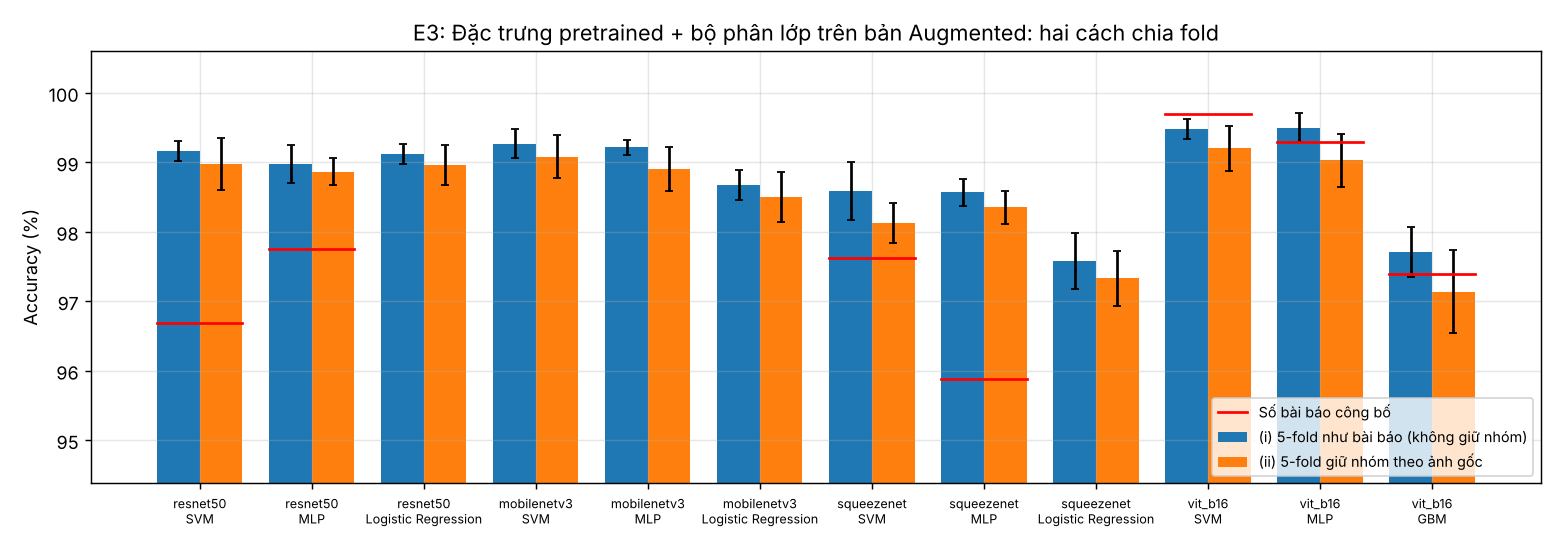
\includegraphics[width=\linewidth,height=0.72\textheight,keepaspectratio]{../results/figures/E3_papers_protocols.png}\end{center}
\end{column}
\end{columns}
\note{Nhóm tái hiện được kết quả chính của bài báo, nhưng khoảng cách ViT so với CNN nhỏ hơn bài báo công bố nhiều (dưới 1 điểm thay vì 3 điểm). Giao thức 5-fold trên bản Augmented có rò rỉ nhỏ nhưng nhất quán. Đặc trưng ViT bền hơn CNN trên bộ kiểm tra khó, đổi lại nặng và chậm hơn khoảng 23 lần. Bảng: results/E3\_bai\_bao/table\_protocols.md, table\_test.md.}
\end{frame}

\begin{frame}{Phụ lục. So sánh bốn nhánh qua cấu hình đại diện}
\begin{center}\begin{adjustbox}{max width=\linewidth,max totalheight=0.74\textheight}
\rowcolors{2}{uitbg}{white}
\begin{tabular}{llllllllll}\toprule
\textbf{Nhánh} & \textbf{Cấu hình đại diện} & \textbf{Ảnh gốc} & \textbf{Nền hoán đổi} & \textbf{V$\times$0.6} & \textbf{V$\times$1.4} & \textbf{Nhiễu $\sigma$=10} & \textbf{Xoay +30$^\circ$} & \textbf{Che 25\%} & \textbf{Điểm bền} \\ \midrule
G: pipeline gốc & b\_mobilenetv3 & 1.000 & 0.794 & 0.919 & 0.890 & 0.989 & 1.000 & 0.659 & 0.875 \\
X-a: xử lý dữ liệu, tiền xử lý lúc suy luận & b\_mobilenetv3 & 0.995 & 0.995 & 0.943 & 0.915 & 0.988 & 0.998 & 0.450 & 0.881 \\
X-b: xử lý dữ liệu, tăng cường có thay nền & b\_mobilenetv3 & 1.000 & 0.975 & 0.954 & 0.935 & 0.995 & 1.000 & 0.441 & 0.883 \\
T: Augmented của tác giả (không rò rỉ) & b\_mobilenetv3 & 0.998 & 0.867 & 0.954 & 0.904 & 0.993 & 1.000 & 0.736 & 0.909 \\
B1: bài báo, trong phạm vi môn học (CNN + bộ phân lớp) & MobileNetV3-Small + SVM tuyến tính & 0.993 & 0.742 & 0.965 & 0.856 & 0.897 & 0.981 & 0.575 & 0.836 \\
B2: bài báo, đúng phương pháp (ViT + SVM) & ViT-B/16 + SVM & 0.997 & 0.857 & 0.990 & 0.978 & 0.986 & 0.978 & 0.728 & 0.919 \\
\bottomrule\end{tabular}
\end{adjustbox}\end{center}
\note{Mỗi nhánh một cấu hình đại diện, chọn theo điểm lúc phát triển. Trên ảnh gốc các nhánh ngang nhau (0 đến vài ảnh sai). Khác biệt nằm ở bộ kiểm tra khó. Bảng: results/so\_sanh\_nhanh/table\_arms.md, table\_stress.md, table\_models.md.}
\end{frame}

\begin{frame}{Phụ lục. So sánh bốn nhánh theo từng phép thử}
\begin{center}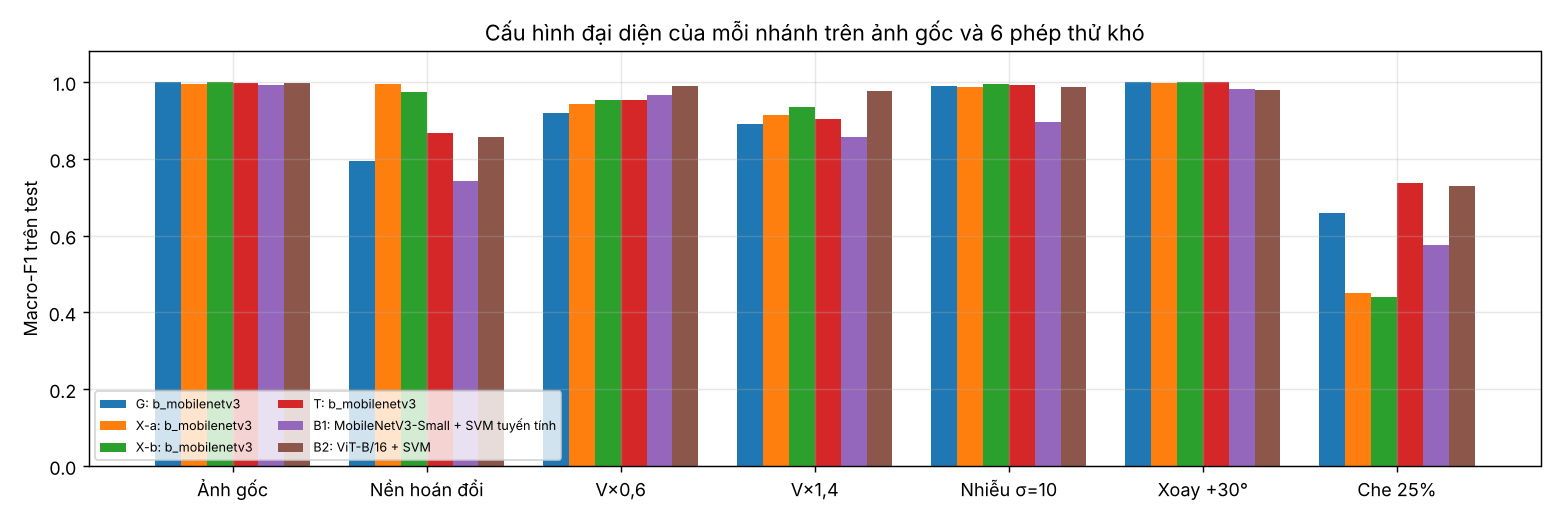
\includegraphics[width=\linewidth,height=0.74\textheight,keepaspectratio]{../results/figures/E_compare_stress.png}\end{center}
\note{Hình cho thấy mỗi nhánh mạnh ở phép thử nào. Không nhánh nào tốt nhất ở mọi phép thử.}
\end{frame}
\end{document}
